

\section{Introduction}

\textcite{pyle2019} introduce a novel learning algorithm to the reservoir computing framework, which harnesses the dynamics of a recurrently connected network to generate time series. Most existing algorithms are built on fully supervised learning rules (e.g. FORCE \cite{sussillo2009}), which limits its potential applications, or the more biologically-realistic reinforcement learning techniques (e.g. RMHL \cite{hoerzer2014}) which unfortunately fail to converge on complex spatio-temporal signal generation tasks. \textcite{pyle2019} utilise the advantages of these two learning rules, while averting their individual shortcomings, by combining the two algorithms to form the SUPERTREX model. The workings of this model are aligned to the theory of motor learning involving the basal ganglia, from both rodent and songbird literature \cite{brainard2002}. It has been hypothesised that a cortical pathway may work in tandem with a pathway via the basal ganglia for motor skill acquisition, wherein the basal ganglia pathway would function as a tutor providing guiding signals, which would ultimately be consolidated in the primary cortical pathway in charge of production of the motor commands \cite{olveczky2011}. Here, the basal ganglia pathway, which uses reward-modulated exploration based learning, akin to the RMHL algorithm, works in parallel with the cortical pathway, modeled using the fully-supervised FORCE algorithm. The SUPERTREX model uses both these pathways in parallel, with the RMHL-based pathway providing the supervisory signal that the FORCE-based pathway requires.
%
In this article, we provide a modular and user-friendly Python re-implementation of the model presented by \textcite{pyle2019}.




\subsection{Framework}

The paper \cite{pyle2019} proposes a model for sensorimotor learning using the framework of reservoir computing. It is based on two existing reservoir computing techniques:- FORCE and RMHL.\\

FORCE (or first-order reduced and controlled error) is a fully-supervised learning rule, which is widely used within the reservoir computing framework \cite{sussillo2009}. A recurrently connected reservoir, composed of rate-coded neurons is trained to produce a target time series by modifying the readout weights between the reservoir and the output layer. The output, in turn, interacts with the reservoir by providing feedback. FORCE can accurately generate complex dynamical target time-series. However, the model must have explicity knowledge of the target function, as FORCE requires a fully supervisory signal of the correct output in order to compute the error during training. \\


RMHL (or Reward-Modulated Hebbian Learning) is built on the concept of reinforcement learning, and uses only a scalar error signal indicating reward, allowing it to be applicable in a wider range of scenarios than FORCE \cite{hoerzer2014}. RMHL introduces perturbations in the performance of the model, and uses the information gained from this exploration to find the target. This is akin to dopamine-dependent Hebbian learning in the basal ganglia. However, RMHL fails to converge to an accurate solution on several complex tasks. Moreover, it has been observed in songbirds that while the basal ganglia provdes a tutor signal in the early stages, learning is eventually consolidated in a parallel cortical pathway, which is primarily responsible for motor activity \cite{olveczky2011}. RMHL cannot account for such empirical observations.\\


SUPERTREX, the model proposed by the authors, tries to merge the advantages of both of these algorithms by combining both models. The more wide-ranged applicability of RMHL, owing to its usage of a one dimensional error signal, is used to train the model, while the superior maintenance ability of FORCE is recruited to consolidate the tutoring of the RMHL pathway. This allows for partially unsupervised learning, along with better performance post-training. This could also potentially explain the empirical evidence, discussed above. Thus, the SUPERTREX model consists of two parallel pathways, one based on RMHL (exploratory) and one based on FORCE (mastery), each consisting of its own set of weights. The mastery pathway uses the output of the exploratory pathway as its supervisory signal.


\begin{equation}
    \mathbf{z}=\mathbf{z}_{1}+\mathbf{z}_{2}
\end{equation}

\begin{equation}
    \tau_{w 1} \frac{d W_{1}}{d t}=\Phi(\hat{e}) \hat{\mathbf{z}} \mathbf{r}^{T}
\end{equation}

\begin{equation}
    \tau_{w 2} \frac{d W_{2}}{d t}=\left(\mathbf{z}-\mathbf{z}_{2}\right) \mathbf{r}^{T} P
\end{equation}
    
where the output $\mathbf{z}$ of the model is the combination of the outputs $\mathbf{z_1}$ and $\mathbf{z_2}$ of the FORCE and RMHL pathways, respectively, $\tau$ is a time constant, $W$ denotes the readout weights of the two pathways, $\mathbf{r}$ is the reservoir activity,  $\Phi(x)$ is a sublinear function that controls when to update the weights, $P$ is a running estimate of the inverse of the correlation matrix of rates and $\hat{x}$  is a high-pass filtered version of $x$.


\subsection{Task}

The authors test the SUPERTREX model on three motor tasks, and compare its performance to those of FORCE and RMHL. Each task uses the paradigm of exploration by a multi-segmented arm, pivoted at a point. The target of each task is to learn to produce a given spatio-temporal signal, under different constraints. Task 1 tests the performance of the model when the target output is known. This task requires the spatiotemporal signal to be produced directly by the model. Thus, the error signal is a direct indicator of the change required in the output of the model, i.e. fully supervisory. Task 2 is more indirect, and tests the performance of the model when the target is unknown, and only a scalar error signal is provided. The task requires the angles between the arm segments to be generated by the model, which would in turn produce the trajectory of the target spatio-temporal signal. In this case, the error signal is not a direct indicator of the change required in the output of the model. A non-linear inverse transformation would be required. It is thus, not a fully supervisory signal, but simply a reinforcement signal. In task 3, the movement of the arm segments are penalised variably. This creates the need to choose one from multiple candidate solutions by optimising the cost of changing the angles between the arm segments.


\subsubsection{Disclaimer}
\textcite{pyle2019} proceed to test the model under variations of the above tasks, including disrupted learning and with additional state information. However, these variations have not been replicated by us. We only test the performance of the three learning rules on the three tasks, specified above.


\section{Comparison with Python Re-implementation}

In this section, we compare the results presented in the paper \cite{pyle2019} with the MATLAB implementation by the authors and our Python re-implementation. The scripts of the authors, although not available online, are readily available on request. We present our adaptation of this model in the open source framework Python, which has been built based on the paper and the MATLAB scripts provided by the authors. In contrast to the author scripts, it is modular and is easily modifiable with external json descriptor files. We compare the results presented in the paper, with simulations of the MATLAB scripts, provided by the author and also with our re-implementation in Python.\\ 

To verify the performance of the model, we test the three algorithms on three tasks by simulating them using both the author scripts and our Python re-implementation. We produce ten simulations with arbitrary seeds initialising the random generator and one additional simulation using the default seed of MATLAB (equivalent to seed 5489 of the numpy random generator). Both MATLAB and numpy use the Mersenne Twister pseudo-random number generator \cite{matsumoto1998}.



\subsection{Task 1}

Here, we compare the simulations of the author scripts and our re-implementation for Task 1 using FORCE, RMHL and SUPERTREX, with the results presented in the article. Task 1 is designed to test the performance of these three algorithms when generating a known target output. The objective of this task is to produce a sequence of 2-D coordinates required to traverse a target time-series, in this case, the parameterized curve of a butterfly. The model is trained to generate an output which closely matches the target function. Post the training phase, the readout weights are frozen and in the SUPERTREX model, the exploratory pathway is deactivated. \\ 

The article claims that :
\begin{itemize}
\item under the FORCE framework, the target time-series is learned accurately and is maintained in a stable manner during the testing phase (Figure~\ref{Fig:compTask1FORCE}).
\item under the RMHL framework, the target time-series is generated accurately during the training phase, however is not maintained perfectly during the testing phase (Figure~\ref{Fig:compTask1RMHL}).
\item under the SUPERTREX framework, the target time-series is learned accurately and is also maintained in a stable manner during testing phase, albeit not as well as FORCE (Figure~\ref{Fig:compTask1ST}).
\end{itemize}

We verify these observations with the MATLAB scripts provided by the authors as well as with our Python adaptation. To do so, we run the simulations with the default seed and repeat it ten times with different seeds to initialise the random number generator.  Both the author scripts and the Python re-implementation are able to successfully closely reproduce the results presented in the paper (Figure~\ref{Fig:Comparison_Task1}).




\begin{figure}

    \centering
    \textbf{MATLAB}\hspace{8em}
    \textbf{Original}\hspace{8em}
    \textbf{Python}
    
    \begin{subfigure}{\textwidth}
        \centering
        
        \textbf{\rotatebox[origin=c]{90}{FORCE}}\begin{subfigure}{\textwidth}
        \centering
    
        
\includegraphics[trim=1.5cm 3cm 1.5cm 3cm, clip=true, height=.2\linewidth]{Figures/MATLAB/FORCE_T1_TimeSeries.png} 
        \hspace{3em}
        
\includegraphics[height=.19\linewidth]{Figures/Orig/FORCE_T1_TimeSeries.png} 
        \hspace{3em}
        
\includegraphics[trim=1.5cm 1.2cm 1.5cm 1.2cm, clip=true,  height=.2\linewidth]{Figures/Python/FORCE_T1_TimeSeries.png}
        
        \end{subfigure}
         
         
        \textbf{\rotatebox[origin=c]{90}{x(t)}}\begin{subfigure}{\textwidth}
        \centering
        
        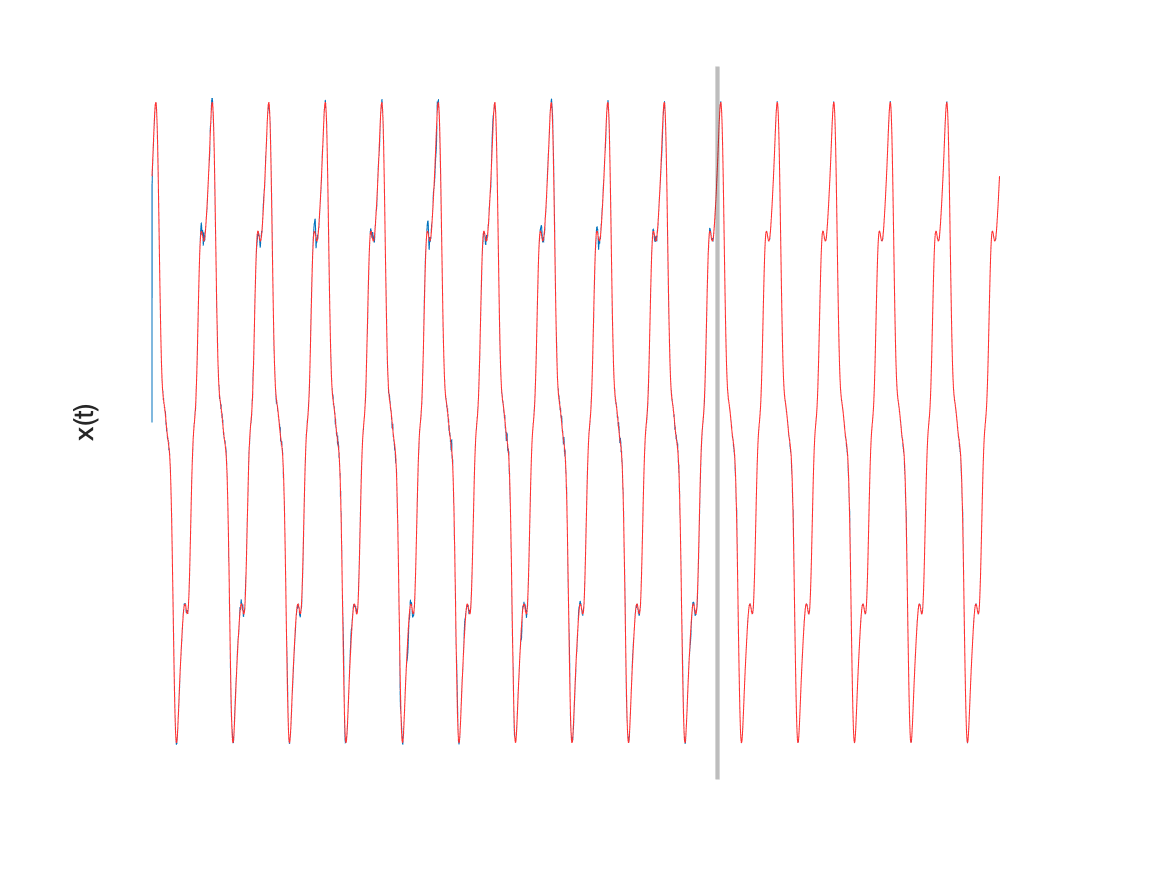
\includegraphics[trim=2cm 0cm 0cm 0cm, clip=true,height=0.1\linewidth,width=.45\linewidth]{Figures/MATLAB/FORCE_T1_CoordinateX.png}
        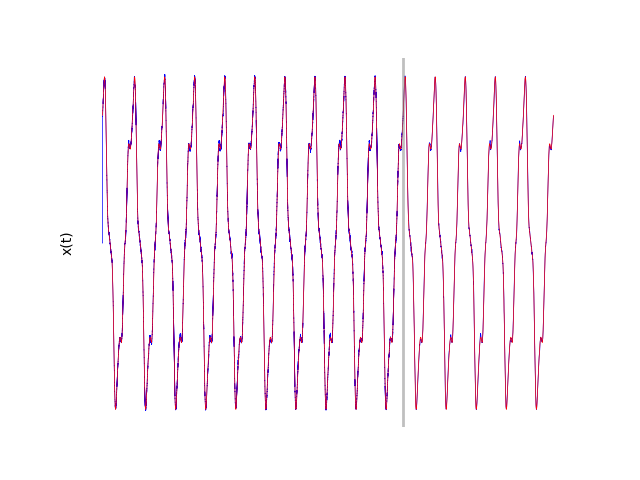
\includegraphics[trim=2cm 0cm 0cm 0cm, clip=true,height=0.1\linewidth,width=.45\linewidth]{Figures/Python/FORCE_T1_CoordinateX.png}
        
        \end{subfigure}
        
        
        \textbf{\rotatebox[origin=c]{90}{y(t)}}\begin{subfigure}{\textwidth}
        \centering
        
        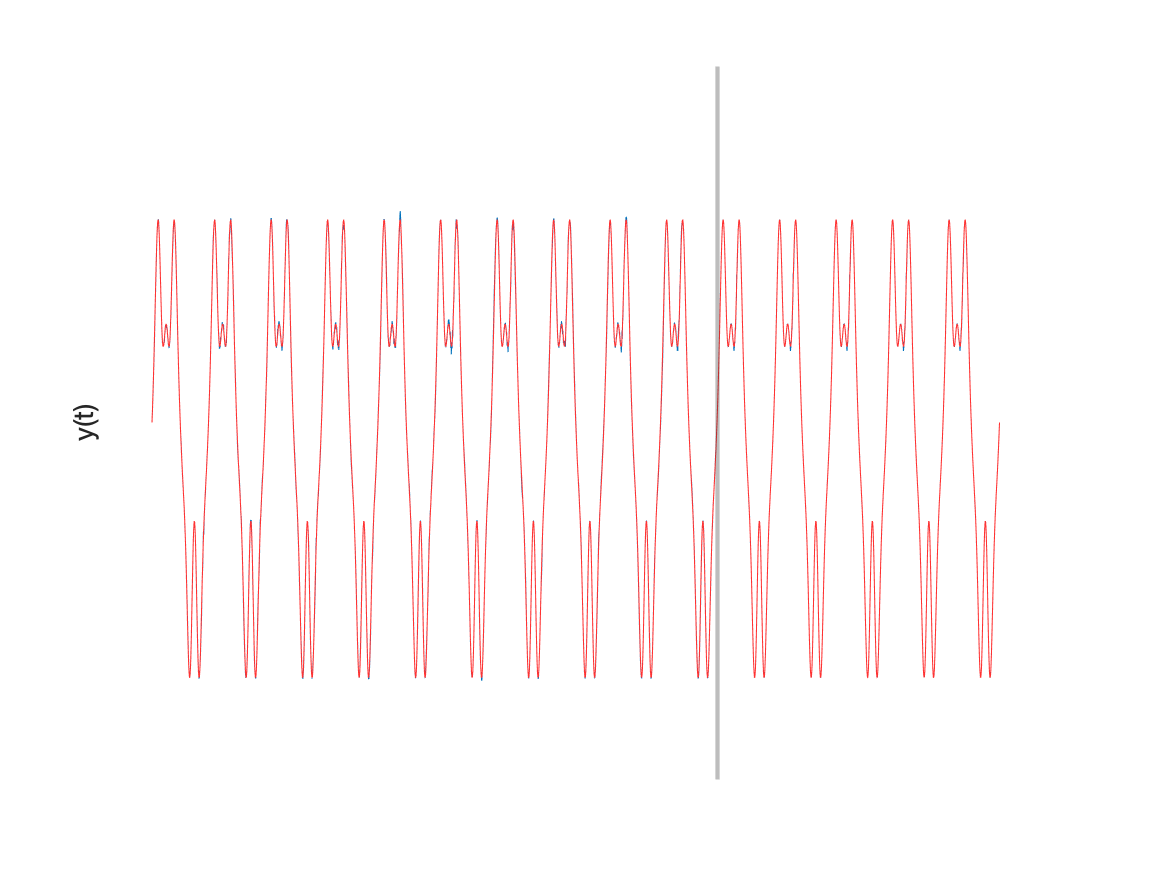
\includegraphics[trim=2cm 0cm 0cm 0cm, clip=true,height=0.1\linewidth,width=.45\linewidth]{Figures/MATLAB/FORCE_T1_CoordinateY.png}
        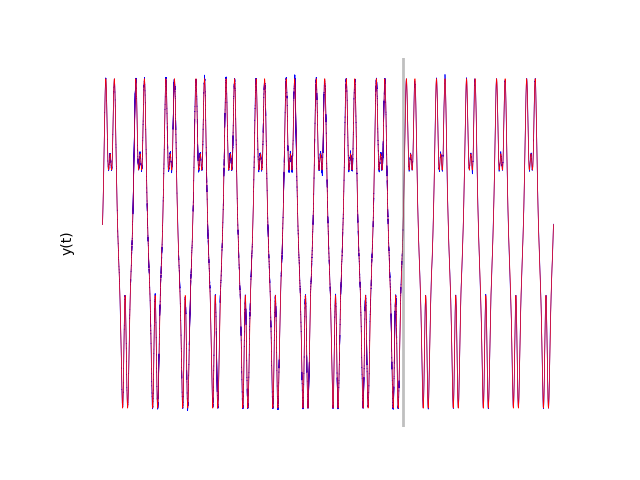
\includegraphics[trim=2cm 0cm 0cm 0cm, clip=true,height=0.1\linewidth,width=.45\linewidth]{Figures/Python/FORCE_T1_CoordinateY.png}
        
        \end{subfigure}
        

    \caption{Results for Task 1 with the FORCE algorithm. The target time‐series is learned accurately during the training phase and is maintained in a stable manner during the testing phase, in both implementations, as presented in \cite{pyle2019}.}
    \label{Fig:compTask1FORCE}
    \end{subfigure}

    \begin{subfigure}{\textwidth}
        \centering
        
        \textbf{\rotatebox[origin=c]{90}{RMHL}}\begin{subfigure}{\textwidth}
        \centering
    
        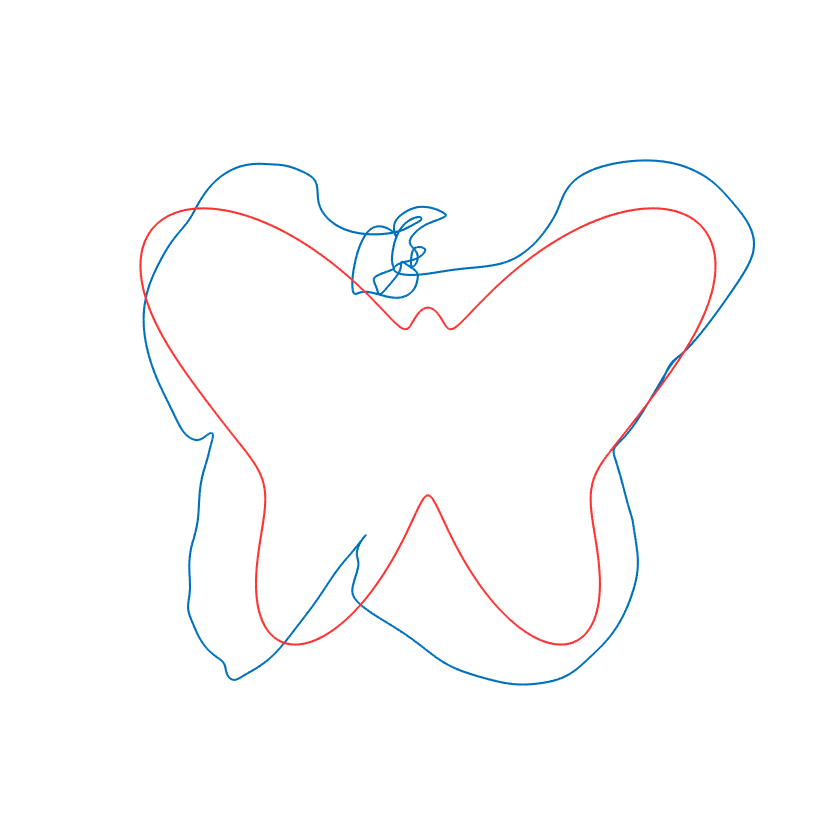
\includegraphics[trim=1.3cm 2cm 1.3cm 2cm, clip=true, height=.2\linewidth]{Figures/MATLAB/RMHL_T1_TimeSeries.png}
        \hspace{3em}
        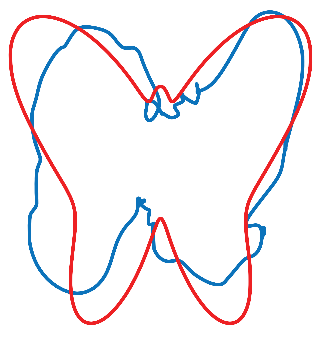
\includegraphics[height=.19\linewidth]{Figures/Orig/RMHL_T1_TimeSeries.png}
        \hspace{3em}
        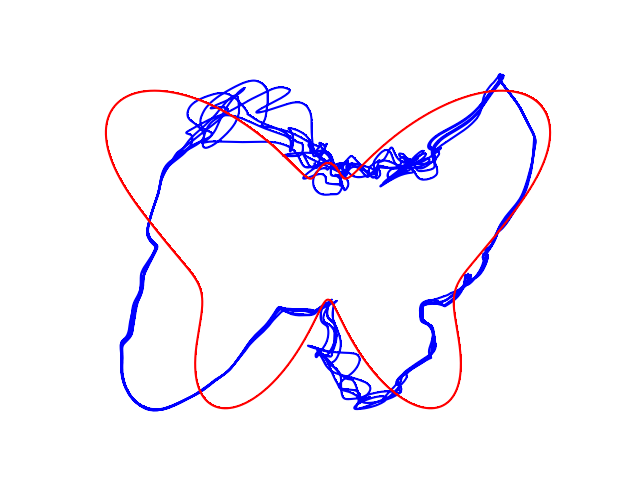
\includegraphics[trim=1.5cm 1.2cm 1.5cm 1.2cm, clip=true,  height=.2\linewidth]{Figures/Python/RMHL_T1_TimeSeries.png}
        
        \end{subfigure}
         
        
        
        \textbf{\rotatebox[origin=c]{90}{x(t)}}\begin{subfigure}{\textwidth}
        \centering
        
        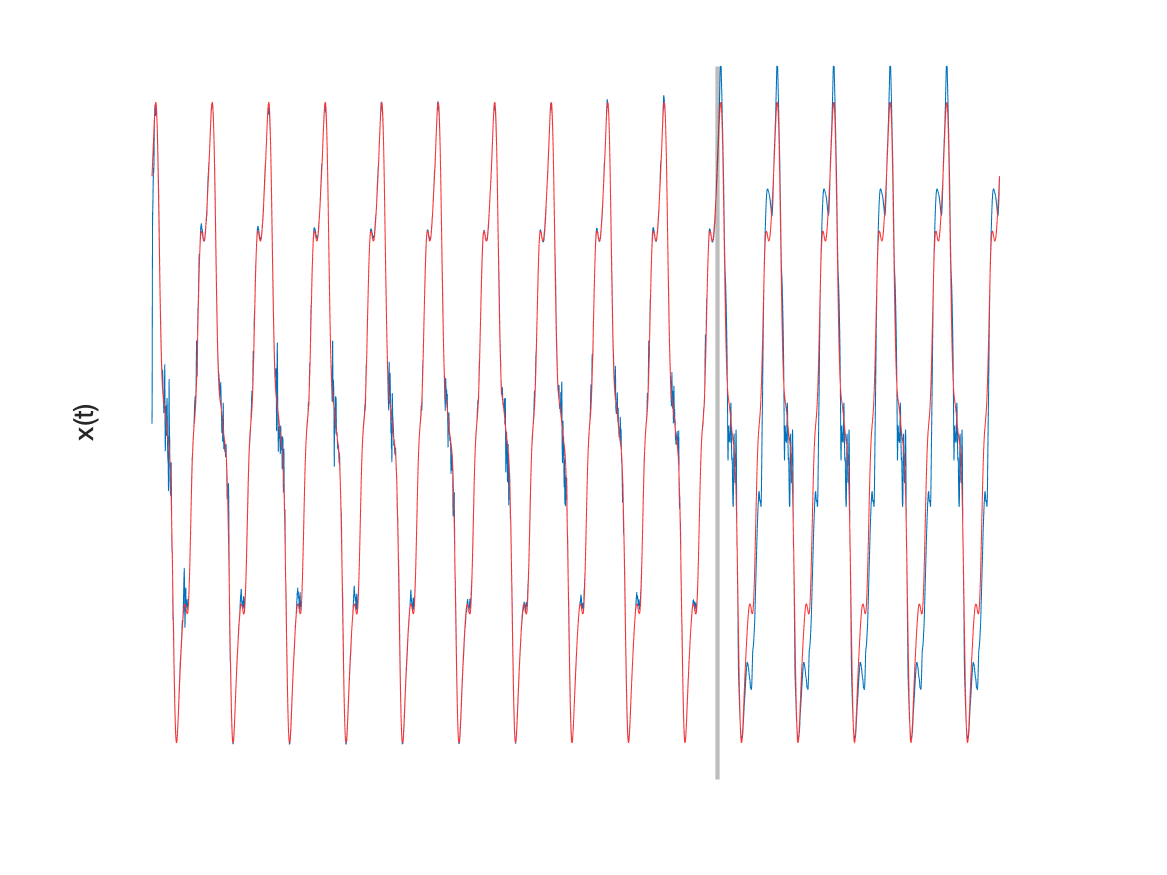
\includegraphics[trim=2cm 0cm 0cm 0cm, clip=true,height=0.1\linewidth,width=.45\linewidth]{Figures/MATLAB/RMHL_T1_CoordinateX.png}
        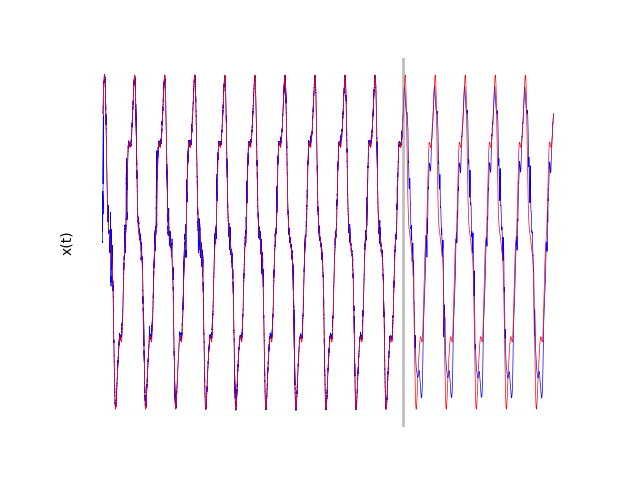
\includegraphics[trim=2cm 0cm 0cm 0cm, clip=true,height=0.1\linewidth,width=.45\linewidth]{Figures/Python/RMHL_T1_CoordinateX.png}
        
        \end{subfigure}
         
        
        
        \textbf{\rotatebox[origin=c]{90}{y(t)}}\begin{subfigure}{\textwidth}
        \centering
        
        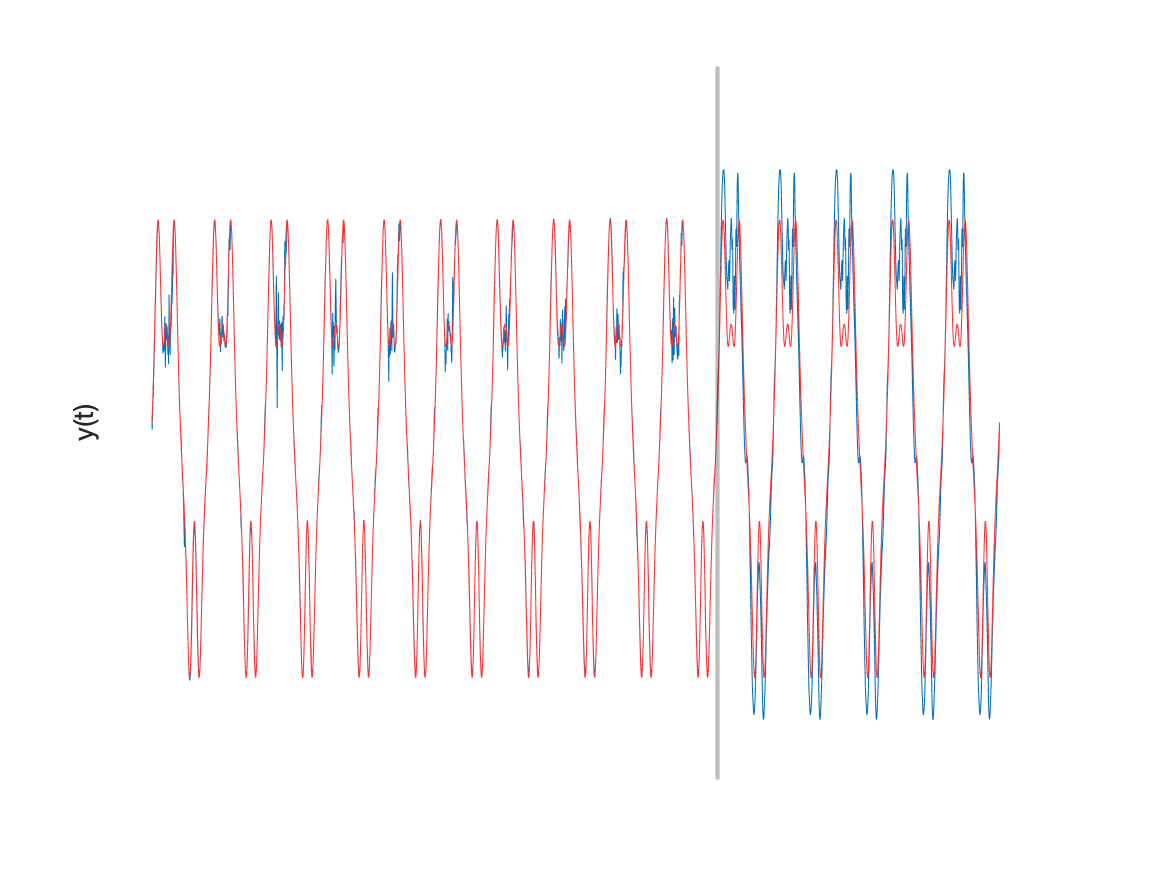
\includegraphics[trim=2cm 0cm 0cm 0cm, clip=true,height=0.1\linewidth,width=.45\linewidth]{Figures/MATLAB/RMHL_T1_CoordinateY.png}
        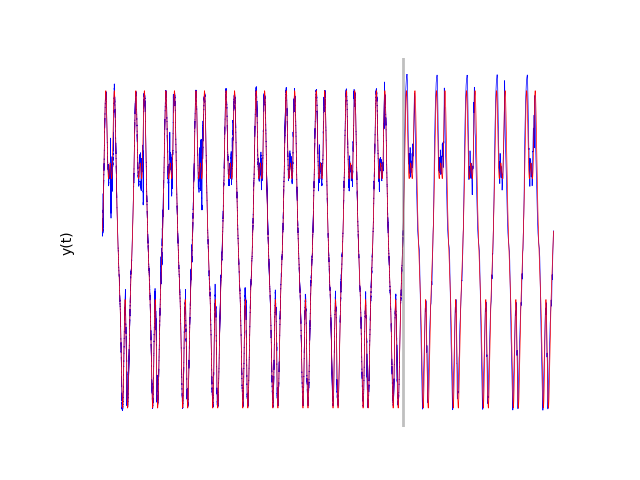
\includegraphics[trim=2cm 0cm 0cm 0cm, clip=true,height=0.1\linewidth,width=.45\linewidth]{Figures/Python/RMHL_T1_CoordinateY.png}
        
        \end{subfigure}
        
    \caption{Results for Task 1 with the RMHL algorithm. The target time‐series is learned accurately during the training phase, however, it is not maintained perfectly during the testing phase, in both implementations, as presented in \cite{pyle2019}.}
    \label{Fig:compTask1RMHL}
    \end{subfigure}
    
    \begin{subfigure}{\textwidth}
        \centering
        
        \textbf{\rotatebox[origin=c]{90}{SUPERTREX}}\begin{subfigure}{\textwidth}
        \centering
    
        
\includegraphics[trim=1.5cm 3cm 1.5cm 3cm, clip=true, height=.2\linewidth]{Figures/MATLAB/ST_T1_TimeSeries.png} 
        \hspace{3em}
        
\includegraphics[height=.19\linewidth]{Figures/Orig/ST_T1_TimeSeries.png}
        \hspace{3em} 
\includegraphics[trim=1.5cm 1.2cm 1.5cm 1.2cm, clip=true,  height=.2\linewidth]{Figures/Python/ST_T1_TimeSeries.png}
        
        \end{subfigure}
         
        
        
        \textbf{\rotatebox[origin=c]{90}{x(t)}}\begin{subfigure}{\textwidth}
        \centering
        
        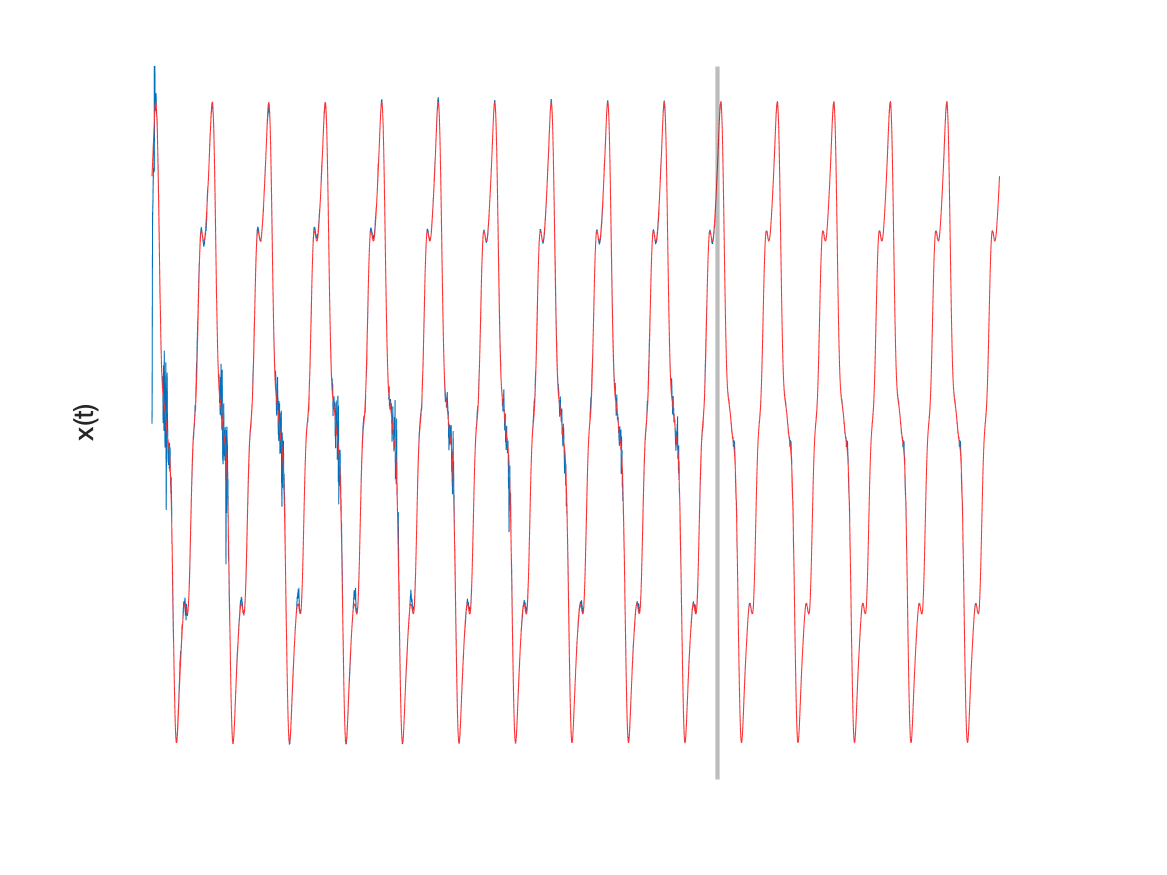
\includegraphics[trim=2cm 0cm 0cm 0cm, clip=true,height=0.1\linewidth,width=.45\linewidth]{Figures/MATLAB/ST_T1_CoordinateX.png}
        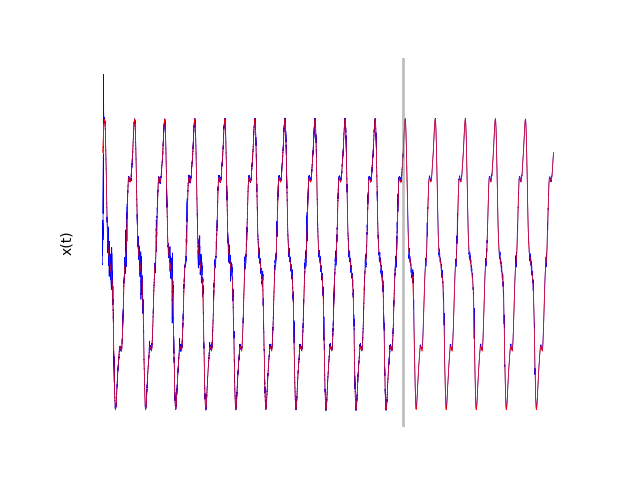
\includegraphics[trim=2cm 0cm 0cm 0cm, clip=true,height=0.1\linewidth,width=.45\linewidth]{Figures/Python/ST_T1_CoordinateX.png}
        
        \end{subfigure}
         
        
        
        \textbf{\rotatebox[origin=c]{90}{y(t)}}\begin{subfigure}{\textwidth}
        \centering
        
        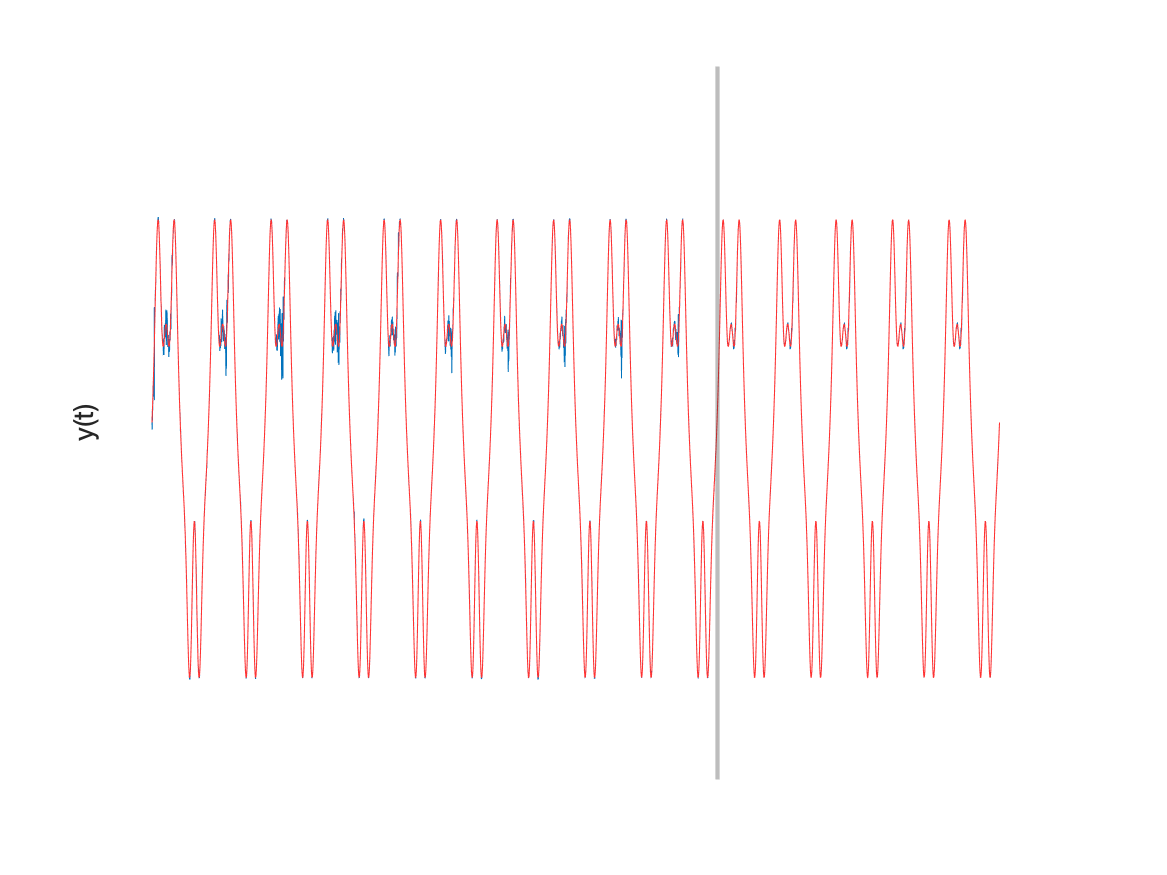
\includegraphics[trim=2cm 0cm 0cm 0cm, clip=true,height=0.1\linewidth,width=.45\linewidth]{Figures/MATLAB/ST_T1_CoordinateY.png}
        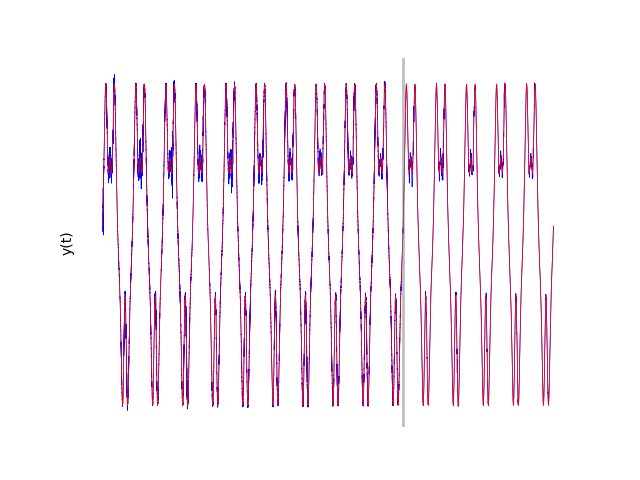
\includegraphics[trim=2cm 0cm 0cm 0cm, clip=true,height=0.1\linewidth,width=.45\linewidth]{Figures/Python/ST_T1_CoordinateY.png}
        
        \end{subfigure}
        

    \caption{Results for Task 1 with the SUPERTREX algorithm. The target time‐series is learned accurately during the training phase, andis also maintained in a stable manner during testing phase, albeit not as well as FORCE, in both implementations, as presented in \cite{pyle2019}.}
    \label{Fig:compTask1ST}
    
    \end{subfigure}


\caption{Comparison of the performances of MATLAB (left column) and Python (right column) implementations with the results presented in the original article (center column), for the three learning algorithms on task 1 \cite{pyle2019}. All simulations shown here use the MATLAB default (5489) as the seed for the random number generator. In each subfigure, the top row shows the target curve (red) with the curve generated by the algorithm (blue) throughout the test phase. The second row shows the actual output (blue) of the model (x and y coordinates, in this case) along with the target output (red), for the corresponding MATLAB (left) and Python (right) simulations. The grey vertical line demarcates the training and testing phase.}
\label{Fig:Comparison_Task1}

\end{figure}



\subsection{Task 2}

We compare the MATLAB scripts and our Python adaptation for the three algorithms on Task 2, with the results presented in the article. Task 2 is designed to test the performance of these three algorithms when generating an unknown target from a scalar error signal. Using the paradigm of a pivoted multi-segmented arm, the objective of this task is to produce a time‐series by generating the angles between the arm segments. Motor output does not control the position of the end-effector of the arm, but instead controls the angles of the arm joints, which are nonlinearly related to end-effector position. Post the training phase, the readout weights are frozen and in the SUPERTREX model, the exploratory pathway is deactivated. \\

The article claims that:
\begin{itemize}
\item the FORCE framework cannot be applied to this task, as FORCE requires the exact target to be provided as a supervisory error, which in this case would be the unknown target angles. Since, we do not have this information beforehand, and require the model to derive it, the FORCE framework is inapplicable to this task.  
\item under the RMHL framework, the target time-series is imitated well by the model during the training phase, however the weights do not converge, and hence, it is unable to maintain the time-series in a stable manner during the testing phase (Figure~\ref{Fig:compTask2RMHL}).
\item under the SUPERTREX framework, the target time-series is learned accurately and is also generated in a stable manner, with minor divergences, during testing phase, owing to the contribution of the pathway based on the FORCE algorithm (Figure~\ref{Fig:compTask2ST}).
\end{itemize}

We verify these observations with the MATLAB scripts provided by the authors as well as with our Python adaptation. To do so, we run the simulations with the default seed of MATLAB and re-simulate it with ten arbitrary seeds to initialise the random number generator. We do not modify any task conditions or model hyper-parameters.  The MATLAB scripts provided by the authors and the Python re-implementation are able to successfully closely reproduce the results presented in the paper with the default seed as well as with the 10 arbitrary seeds (Figure~\ref{Fig:Comparison_Task2}).





\begin{figure}

    \centering
    \textbf{MATLAB}\hspace{8em}
    \textbf{Original}\hspace{8em}
    \textbf{Python}
    

    \begin{subfigure}{\textwidth}
        \centering
        
        \textbf{\rotatebox[origin=c]{90}{RMHL}}\begin{subfigure}{\textwidth}
        \centering
        
        
        \hspace{-2em}
        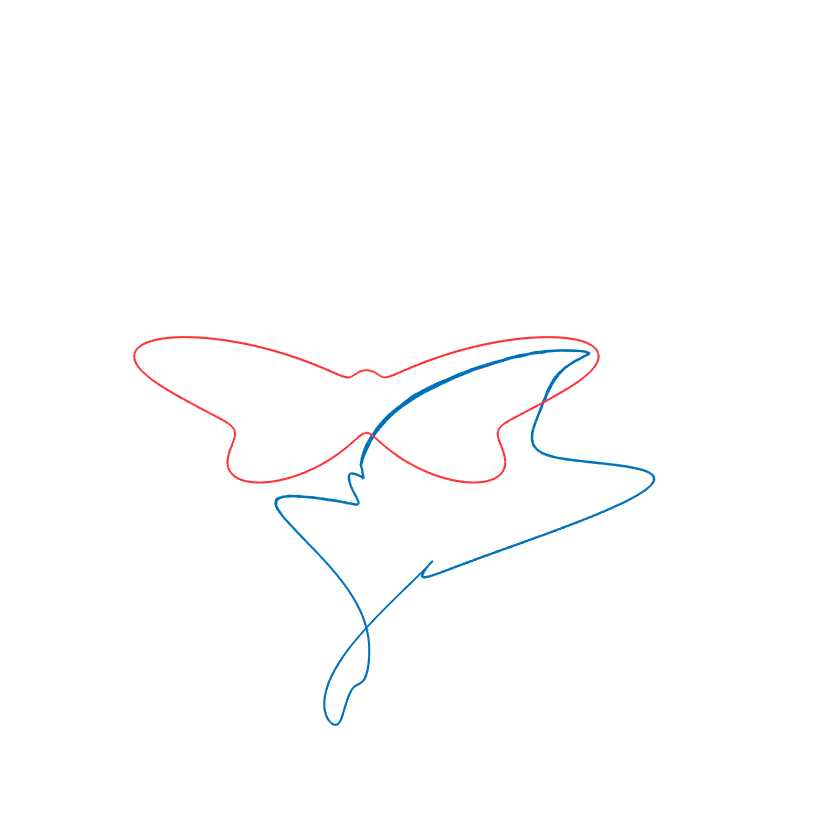
\includegraphics[trim=1.3cm 1.5cm 1.3cm 5.7cm, clip=true, height=.2\linewidth]{Figures/MATLAB/RMHL_T2_Seg2_TimeSeries.png}
        \hspace{-2em}
        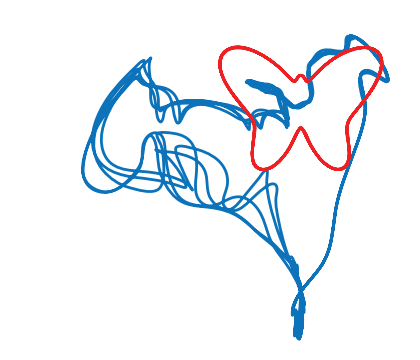
\includegraphics[height=.25\linewidth]{Figures/Orig/RMHL_T2_TimeSeries.png}
        \hspace{.25em}
        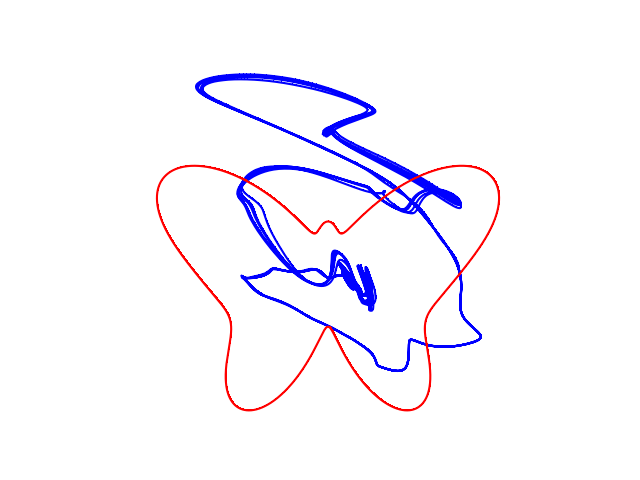
\includegraphics[trim=2cm 0cm 1.5cm 2cm, clip=true,  height=.2\linewidth]{Figures/Python/RMHL_T2_Seg2_TimeSeries.png} 
        
        \end{subfigure}
         
        
        \textbf{\rotatebox[origin=c]{90}{$\theta_1$}}\begin{subfigure}{\textwidth}
        \centering
        
        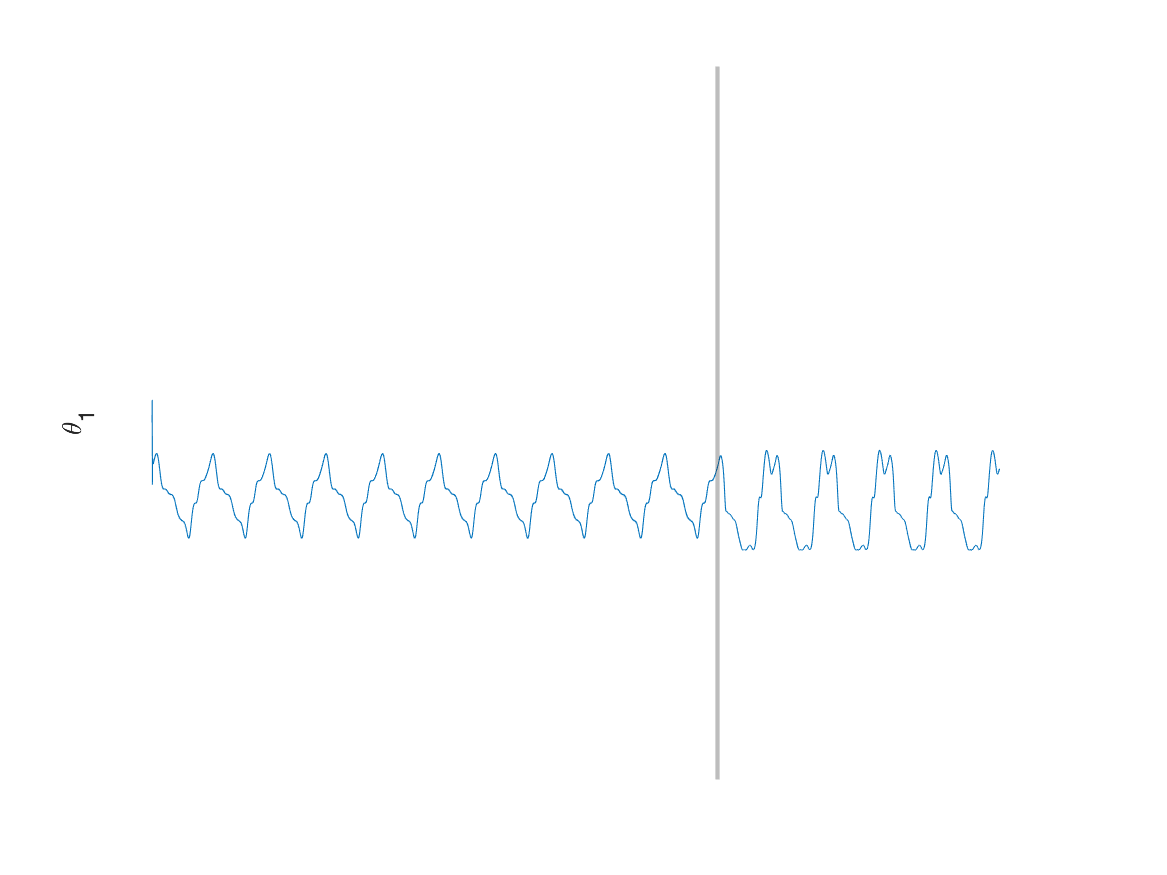
\includegraphics[trim=2cm 0cm 0cm 0cm, clip=true,height=0.1\linewidth,width=.45\linewidth]{Figures/MATLAB/RMHL_T2_Seg2_Theta1.png}
        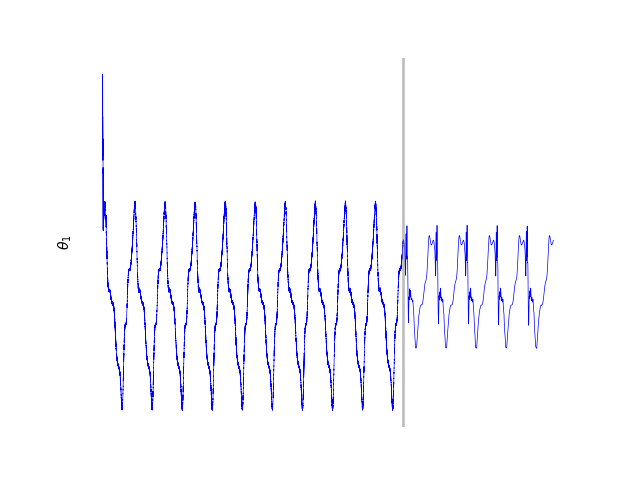
\includegraphics[trim=2cm 0cm 0cm 0cm, clip=true,height=0.1\linewidth,width=.45\linewidth]{Figures/Python/RMHL_T2_Seg2_Theta1.png}
        
        \end{subfigure}
         
        
        \textbf{\rotatebox[origin=c]{90}{$\theta_2$}}\begin{subfigure}{\textwidth}
        \centering
        
        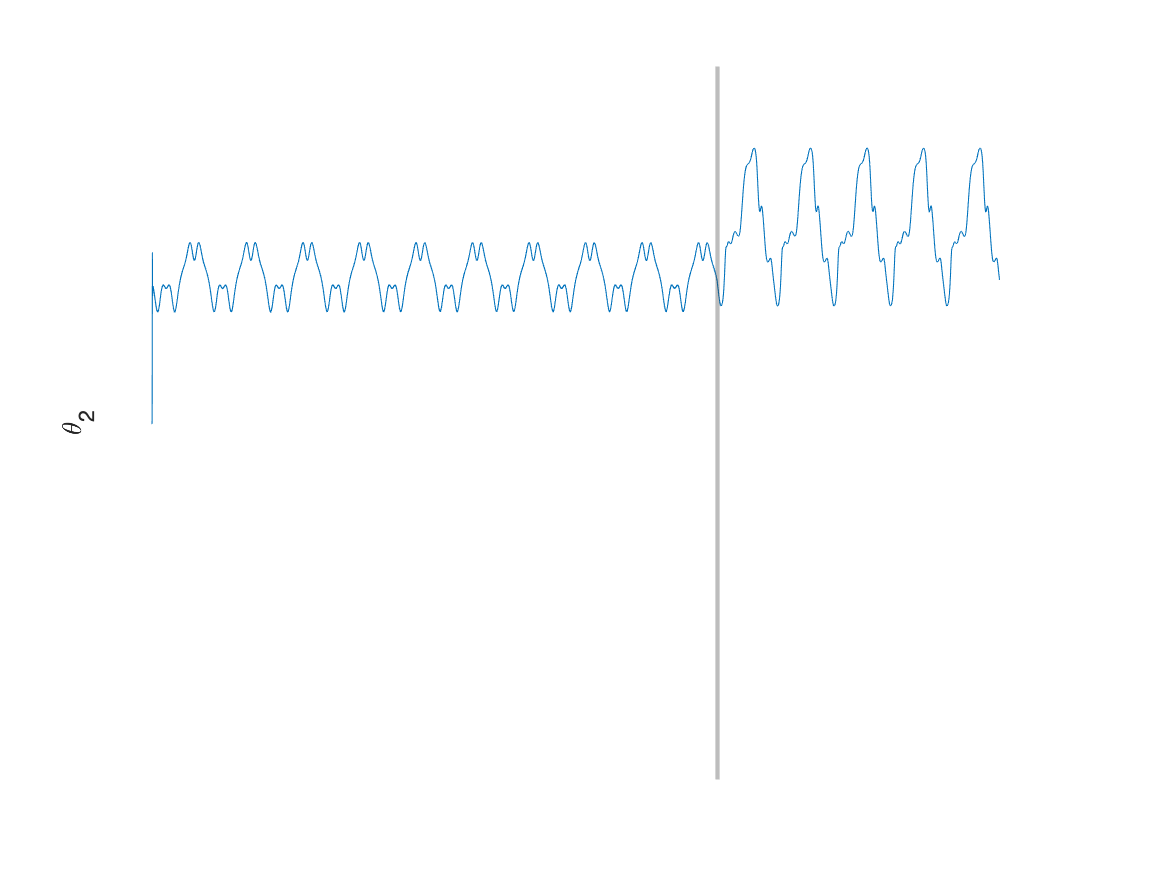
\includegraphics[trim=2cm 0cm 0cm 0cm, clip=true,height=0.1\linewidth,width=.45\linewidth]{Figures/MATLAB/RMHL_T2_Seg2_Theta2.png}
        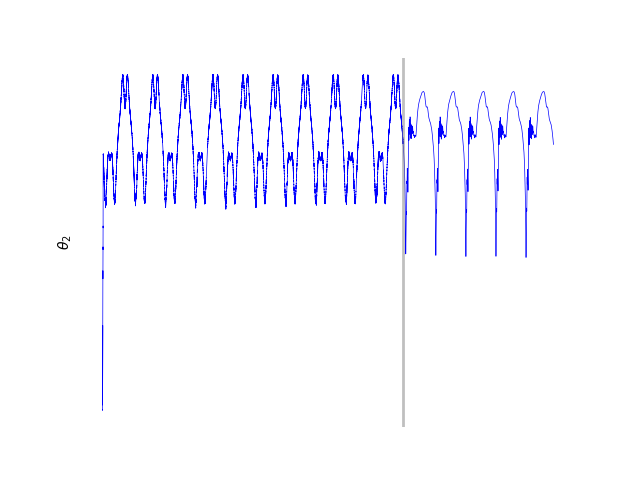
\includegraphics[trim=2cm 0cm 0cm 0cm, clip=true,height=0.1\linewidth,width=.45\linewidth]{Figures/Python/RMHL_T2_Seg2_Theta2.png}
        
        \end{subfigure}
        
    \caption{Results for Task 2 with the RMHL algorithm. The target time‐series is imitated well by the model during the training phase, however, it is unable to maintain the timeseries in a stable manner during the testing phase, in both implementations, as presented in \cite{pyle2019}.}
    \label{Fig:compTask2RMHL}
    \end{subfigure}
    
    \begin{subfigure}{\textwidth}
        \centering
        
        \textbf{\rotatebox[origin=c]{90}{SUPERTREX}}\begin{subfigure}{\textwidth}
        \centering
        
        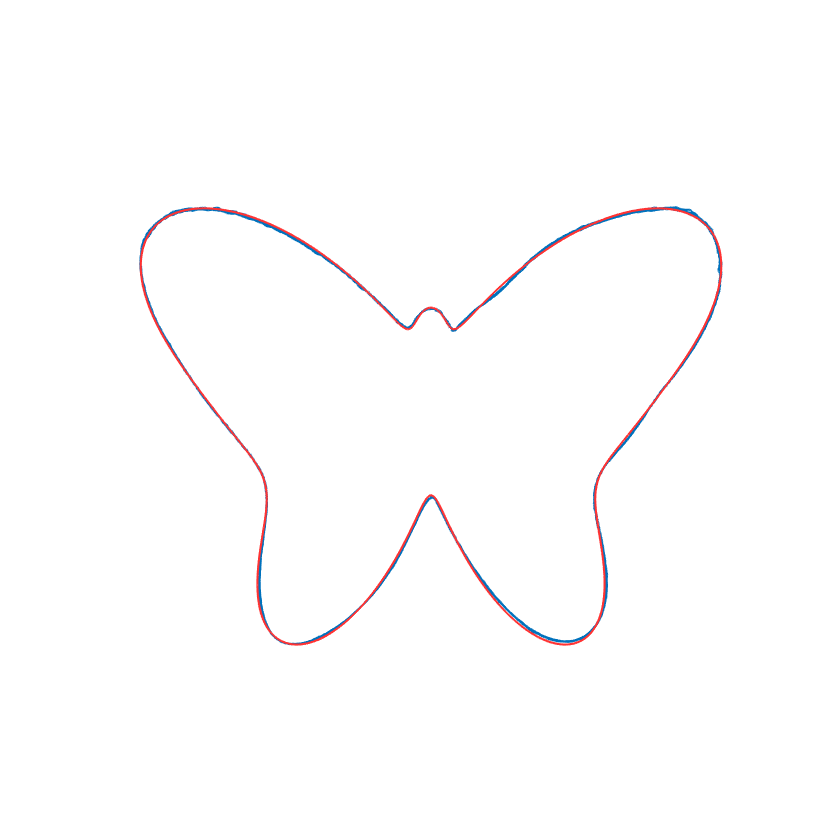
\includegraphics[trim=1.5cm 2.7cm 1.5cm 0.5cm, clip=true, height=.25\linewidth]{Figures/MATLAB/ST_T2_Seg2_TimeSeries.png} 
        \hspace{2em}
        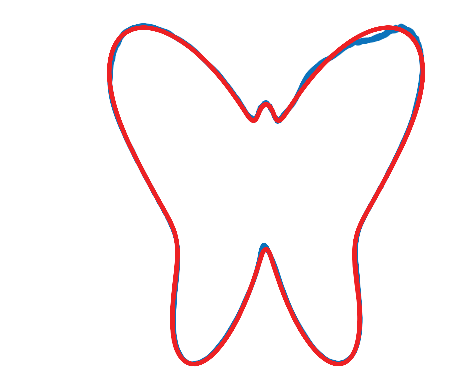
\includegraphics[height=.2\linewidth]{Figures/Orig/ST_T2_TimeSeries.png} 
        \hspace{2em}
        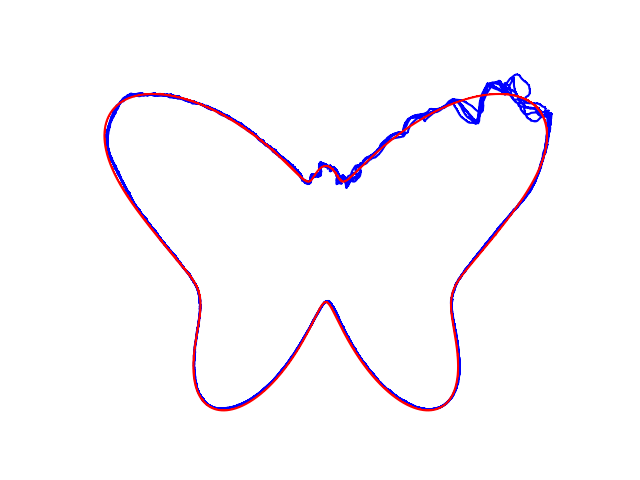
\includegraphics[trim=1.5cm 1.2cm 1.5cm 1.2cm, clip=true,  height=.2\linewidth]{Figures/Python/ST_T2_Seg2_TimeSeries.png} 
        
        \end{subfigure}
        
        
        \textbf{\rotatebox[origin=c]{90}{$\theta_1$}}\begin{subfigure}{\textwidth}
        \centering
        
        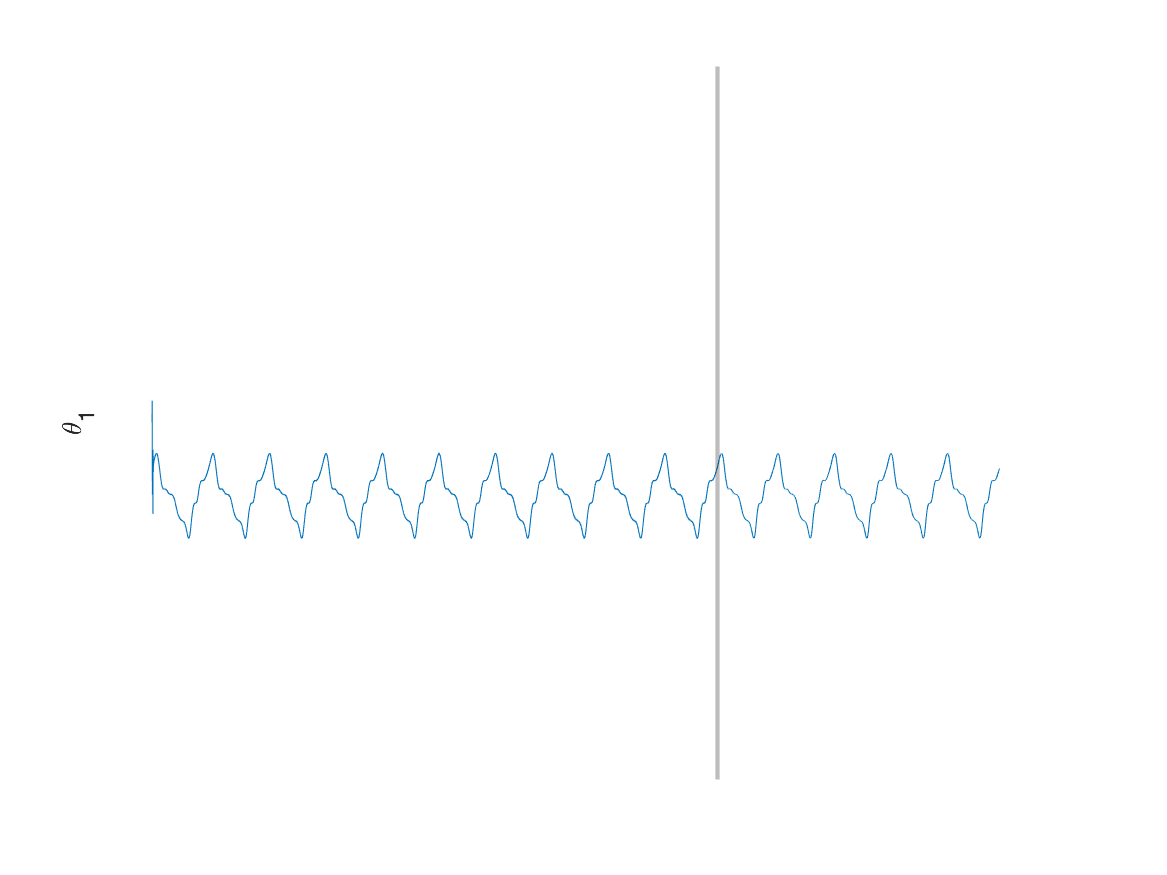
\includegraphics[trim=2cm 0cm 0cm 0cm, clip=true,height=0.1\linewidth,width=.45\linewidth]{Figures/MATLAB/ST_T2_Seg2_Theta1.png}
        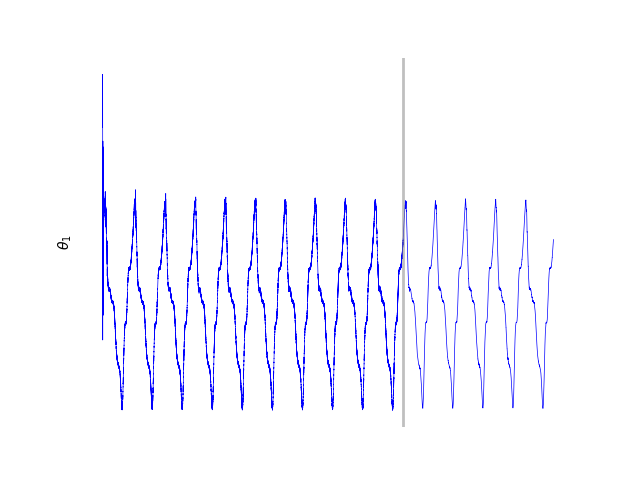
\includegraphics[trim=2cm 0cm 0cm 0cm, clip=true,height=0.1\linewidth,width=.45\linewidth]{Figures/Python/ST_T2_Seg2_Theta1.png}
        
        \end{subfigure}
        
        
        \textbf{\rotatebox[origin=c]{90}{$\theta_2$}}\begin{subfigure}{\textwidth}
        \centering
        
        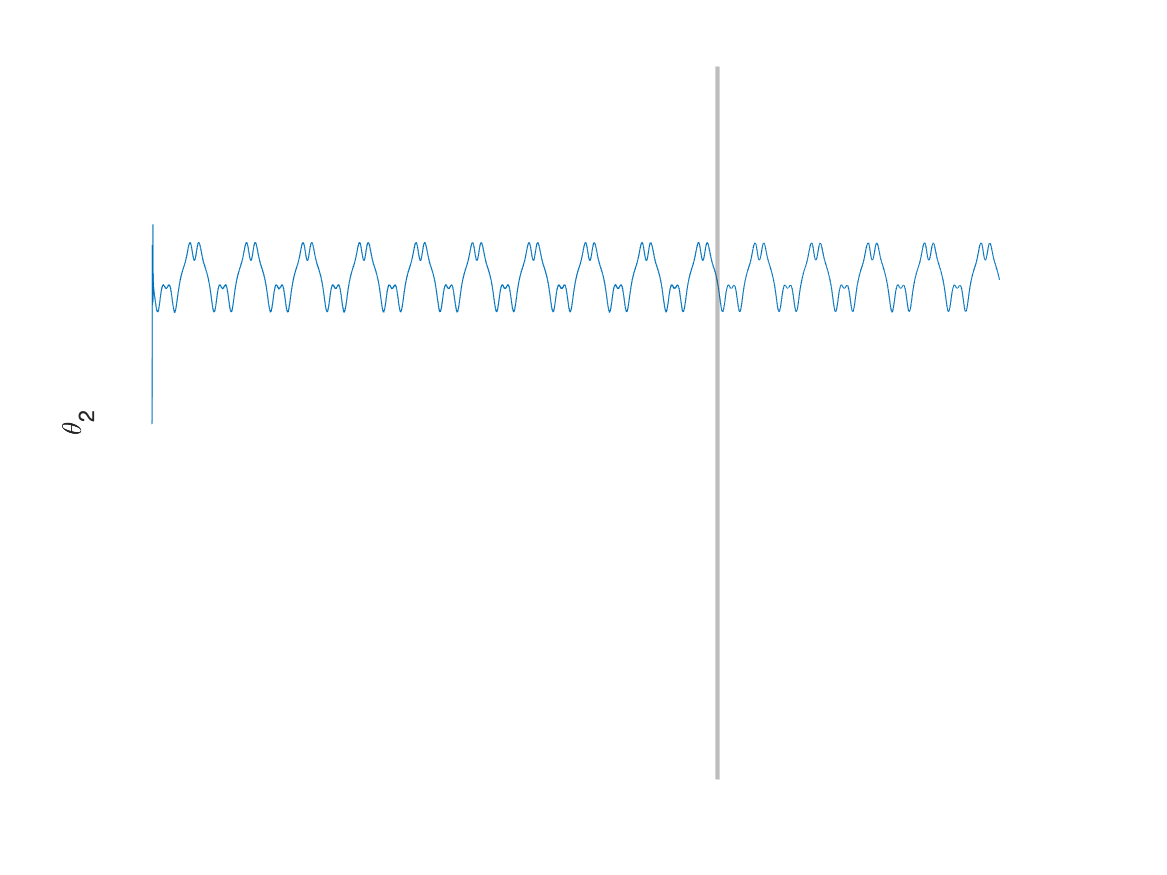
\includegraphics[trim=2cm 0cm 0cm 0cm, clip=true,height=0.1\linewidth,width=.45\linewidth]{Figures/MATLAB/ST_T2_Seg2_Theta2.png}
        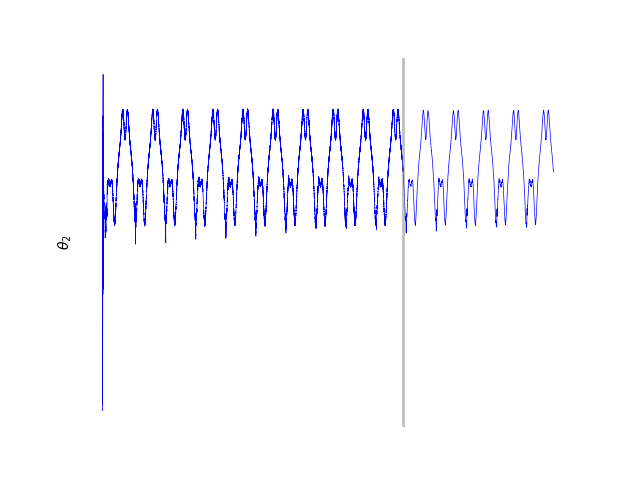
\includegraphics[trim=2cm 0cm 0cm 0cm, clip=true,height=0.1\linewidth,width=.45\linewidth]{Figures/Python/ST_T2_Seg2_Theta2.png}
        
        \end{subfigure}
        

    \caption{Results for Task 2 with the SUPERTREX algorithm. The target time‐series is learned accurately during the training phase, and is also maintained in a stable manner, during the testing phase, in both implementations, as presented in \cite{pyle2019}.}
    \label{Fig:compTask2ST}
    
    \end{subfigure}


\caption{Comparison of the performances of MATLAB (left column) and Python (right column) implementations with the results presented in the original article (center column), for the three learning algorithms on task 2 \cite{pyle2019}. All simulations shown here use the MATLAB default (5489) as the seed for the random number generator. In each subfigure, the top row shows the target curve (red) with the curve generated by the algorithm (blue) throughout the test phase. The second row shows the actual output (blue) of the model (x and y coordinates, in this case) along with the target output (red), for the corresponding MATLAB (left) and Python (right) simulations. The grey vertical line demarcates the training and testing phase.}
\label{Fig:Comparison_Task2}

\end{figure}



\subsection{Task 3}
We compare the performance of the MATLAB scripts and our Python adaptation for the three algorithms  on Task 2, with the results presented in the article. Task 3 is an extension of Task 2, designed to test the constraint optimisation ability of these three algorithms when generating an unknown target from a scalar error signal. Using the paradigm of a pivoted multi-segmented arm, the objective of this task is to produce a time‐series by generating the angles between the arm segments, while also optimising the movement cost of each arm segment. Hence, the arm is required to traverse the butterfly, while carefully choosing the segment to rotate, in order to minimise the movement cost of its segments. Post the training phase, the readout weights are frozen and in the SUPERTREX model, the exploratory pathway is deactivated. \\

The article claim that
\begin{itemize}
    \item FORCE can't be applied to this task, as explained for Task 2.
    \item under the RMHL framework, the target time-series is imitated well by the model during the training phase, however the weights do not converge, and hence, it poorly maintains the time-series during the testing phase (Figure~\ref{Fig:compTask3RMHL}).
    \item under the SUPERTREX framework, the performance is much better than RMHL. The target time-series is learned accurately and is also generated with minor divergences, during testing phase (Figure~\ref{Fig:compTask3ST}).
\end{itemize}

We verify these observations with the MATLAB scripts provided by the authors as well as with our Python adaptation. To do so, we run the simulations with the default seed of MATLAB and re‐simulate it with ten arbitrary seeds to initialise the random number generator. The MATLAB scripts and the Python re-implementation are able to successfully reproduce the results presented in the paper with the default seed as well as with the 10 arbitrary seeds for the RMHL algorithm. The SUPERTREX model does reproduce the results presented in the paper for approximately 50\% of the tested simulations. However, the SUPERTREX model does not robustly perform as presented for the default MATLAB seed (5489), and for 5 out of the 10 additional arbitrary seeds. For these simulations, either the time-series is not maintained during the test phase, or the weights increase uncontrollably, rendering the simulation unable to progress in a meaningful manner (Figure~\ref{Fig:Comparison_Task3}).



\begin{figure}

    \centering
    \textbf{MATLAB}\hspace{8em}
    \textbf{Original}\hspace{8em}
    \textbf{Python}
    

    \begin{subfigure}{\textwidth}
        \centering
        
        \textbf{\rotatebox[origin=c]{90}{RMHL}}\begin{subfigure}{\textwidth}
        \centering
        
        
        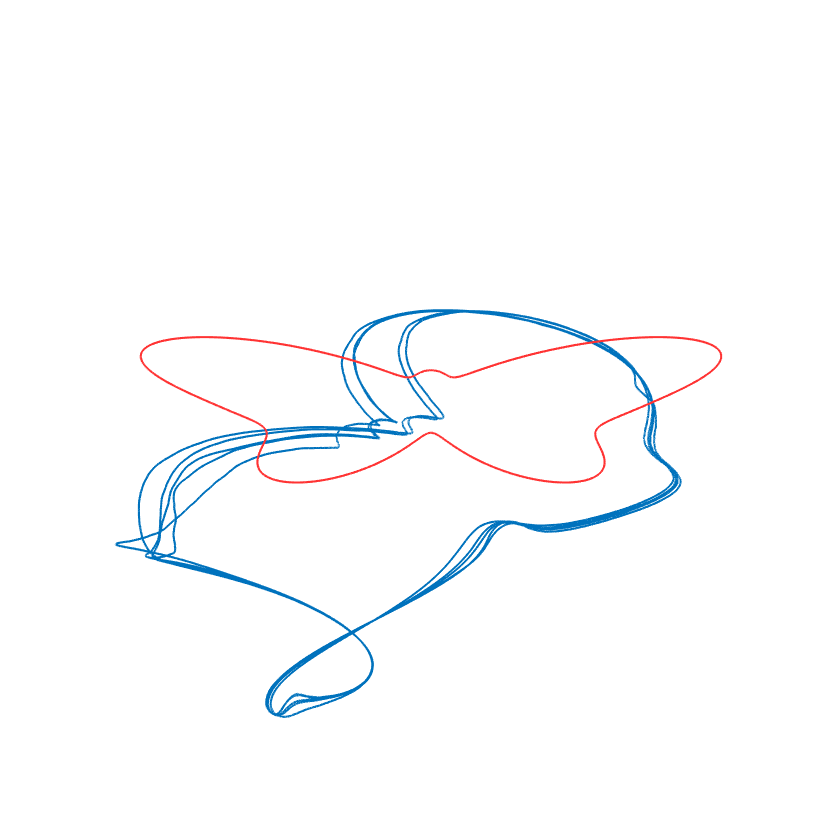
\includegraphics[trim=1.3cm 2cm 1.3cm 2cm, clip=true, height=.25\linewidth]{Figures/MATLAB/RMHL_T3_TimeSeries.png} 
        \hspace{.5em}
        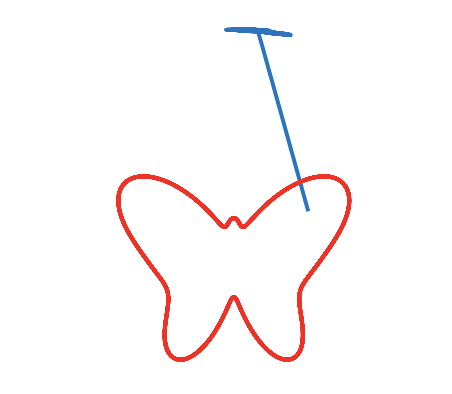
\includegraphics[height=.25\linewidth]{Figures/Orig/RMHL_T3_TimeSeries.png} 
        \hspace{.25em}
        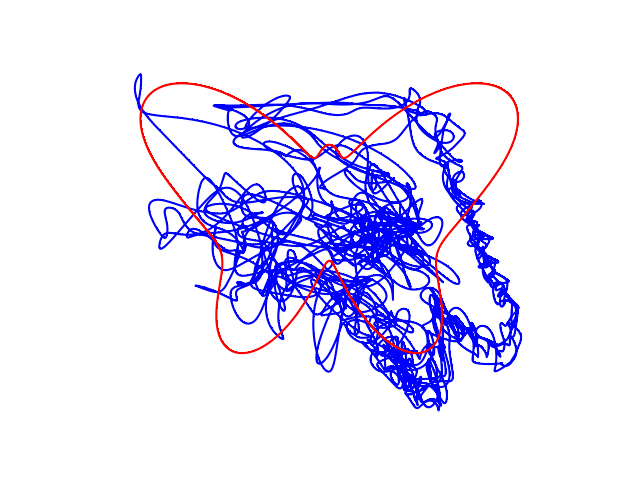
\includegraphics[trim=1.5cm 1.2cm 1.5cm 1.2cm, clip=true,  height=.17\linewidth]{Figures/Python/RMHL_T3_TimeSeries.png}
        
        \end{subfigure}
         
        
        
    \caption{Results for Task 3 with the RMHL algorithm, using the default seed (5489) for the random number generator. The target time‐series is imitated well by the model during the training phase, however, it poorly maintains the timeseries during the testing phase, in both implementations, as presented in \cite{pyle2019}.}
    \label{Fig:compTask3RMHL}
    \end{subfigure}
    
    \begin{subfigure}{\textwidth}
        \centering
        
        \textbf{\rotatebox[origin=c]{90}{SUPERTREX}}\begin{subfigure}{\textwidth}
        \centering
        
        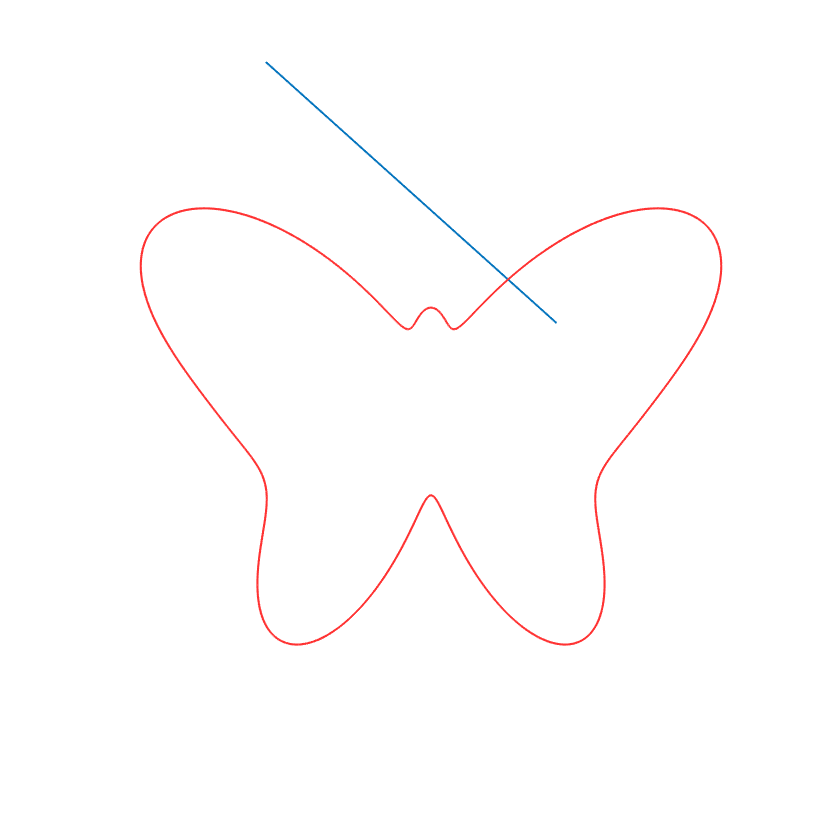
\includegraphics[trim=0.5cm 2.2cm 1.5cm 0cm, clip=true, height=.25\linewidth]{Figures/MATLAB/ST_T3_TimeSeries.png} 
        \hspace{2em}
        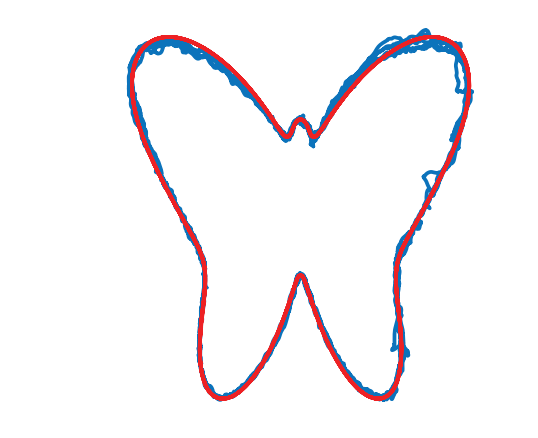
\includegraphics[ height=.18\linewidth]{Figures/Orig/ST_T3_TimeSeries.png}
        \hspace{0em}
        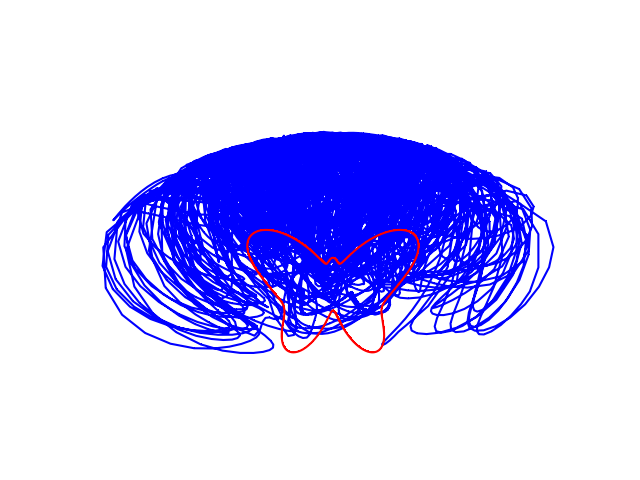
\includegraphics[trim=1.5cm 2.5cm 1.5cm 1.2cm, clip=true,  height=.23\linewidth]{Figures/Python/ST_T3_TimeSeries.png} 
        
        \end{subfigure}
        
        
        \textbf{\rotatebox[origin=c]{90}{$\theta_1$}}\begin{subfigure}{\textwidth}
        \centering
        
        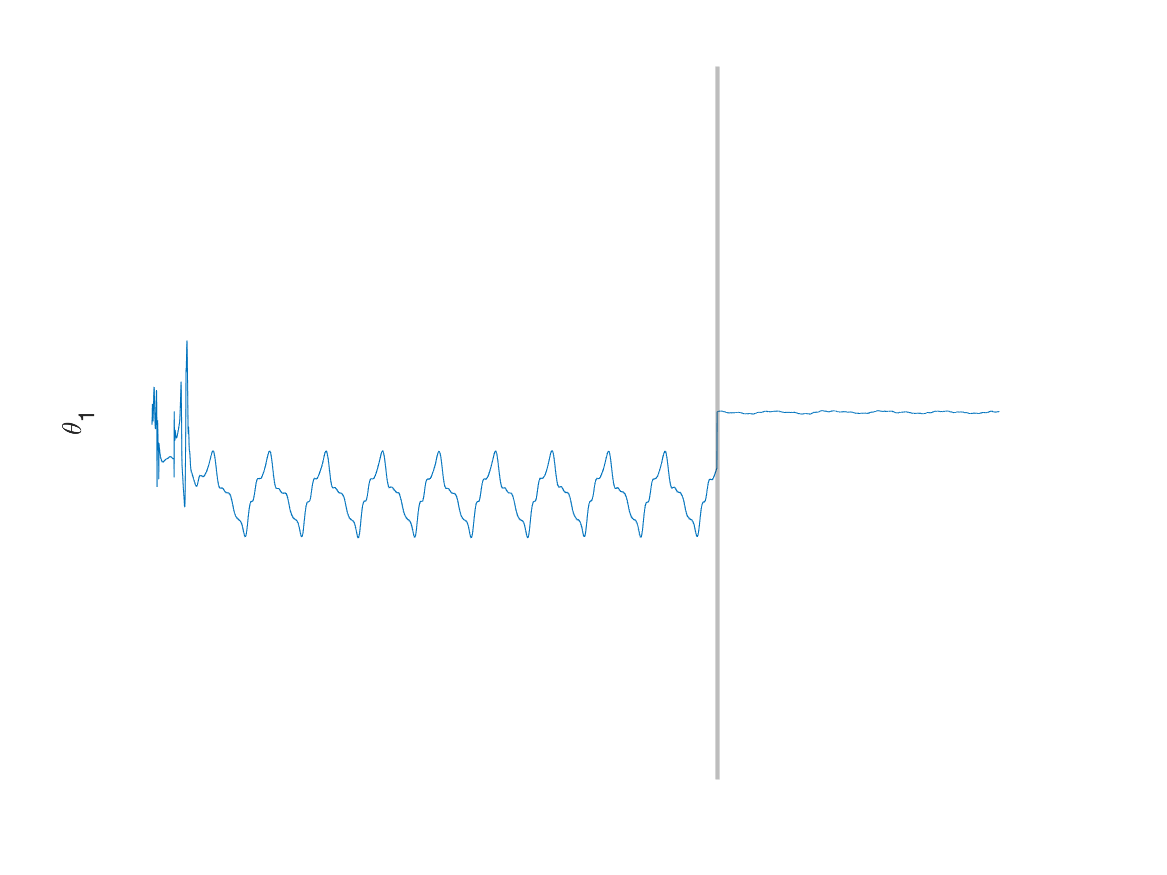
\includegraphics[height=0.1\linewidth,width=.45\linewidth]{Figures/MATLAB/ST_T3_Theta1.png}
        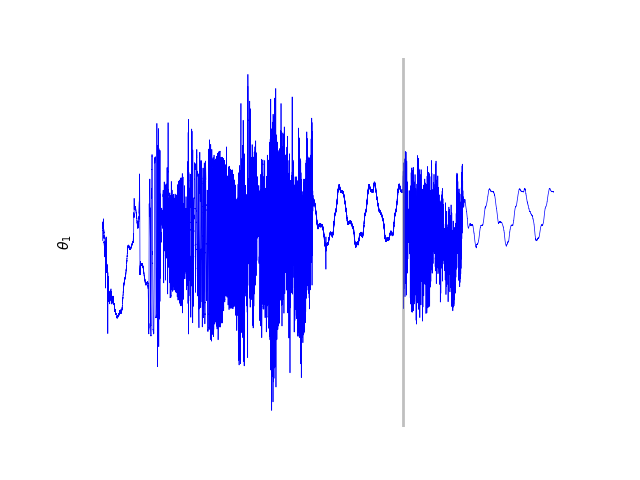
\includegraphics[height=0.1\linewidth,width=.45\linewidth]{Figures/Python/ST_T3_Theta1.png}
        
        \end{subfigure}
        
        
        \textbf{\rotatebox[origin=c]{90}{$\theta_2$}}\begin{subfigure}{\textwidth}
        \centering
        
        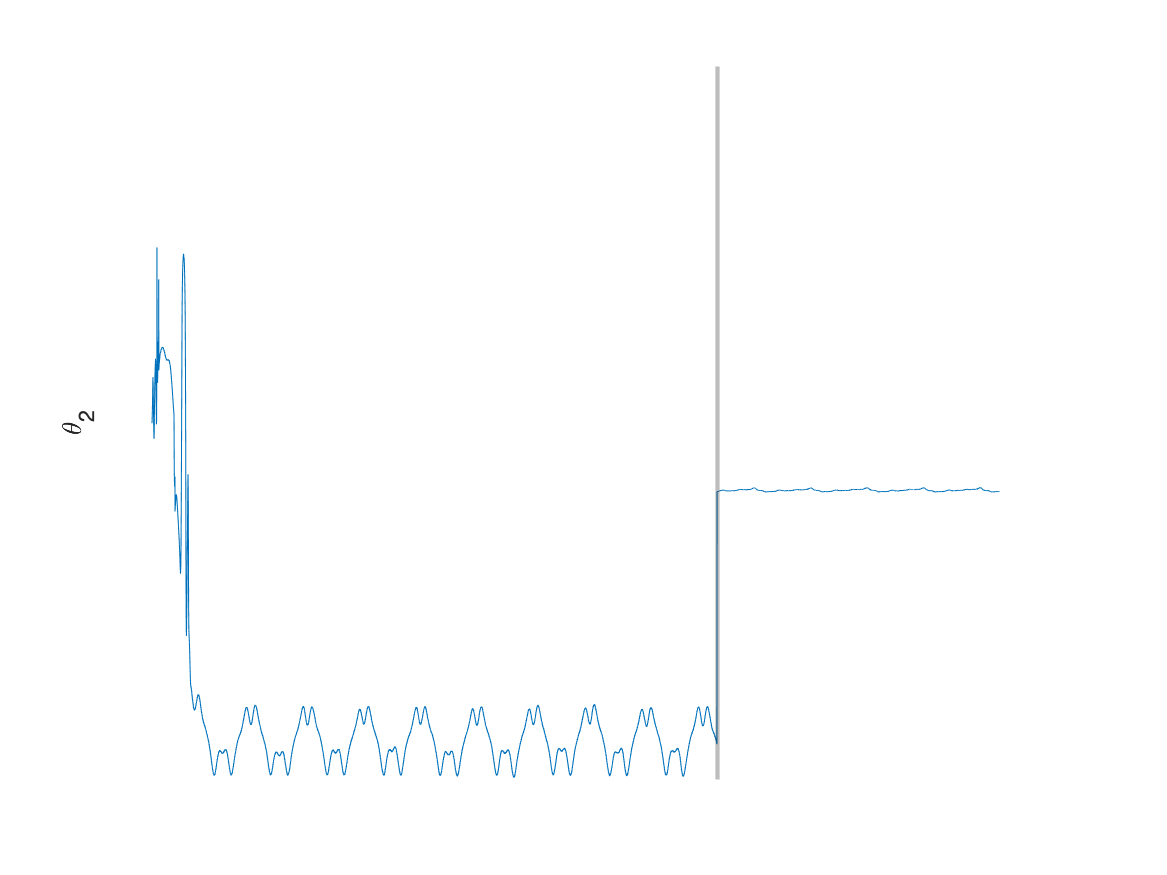
\includegraphics[height=0.1\linewidth,width=.45\linewidth]{Figures/MATLAB/ST_T3_Theta2.png}
        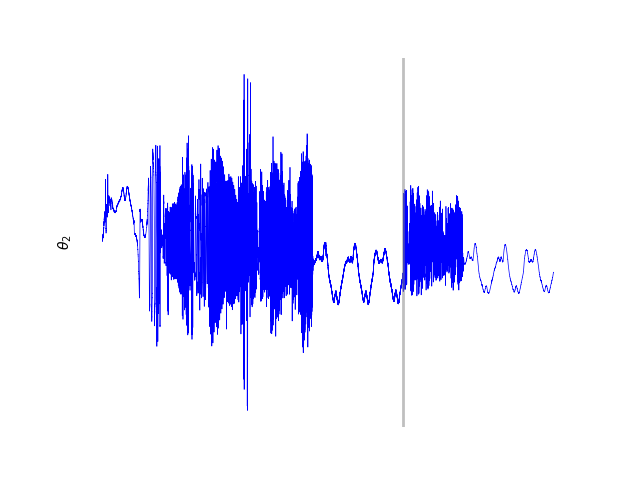
\includegraphics[height=0.1\linewidth,width=.45\linewidth]{Figures/Python/ST_T3_Theta2.png}
        
        \end{subfigure}
        
        
        \textbf{\rotatebox[origin=c]{90}{$\theta_3$}}\begin{subfigure}{\textwidth}
        \centering
        
        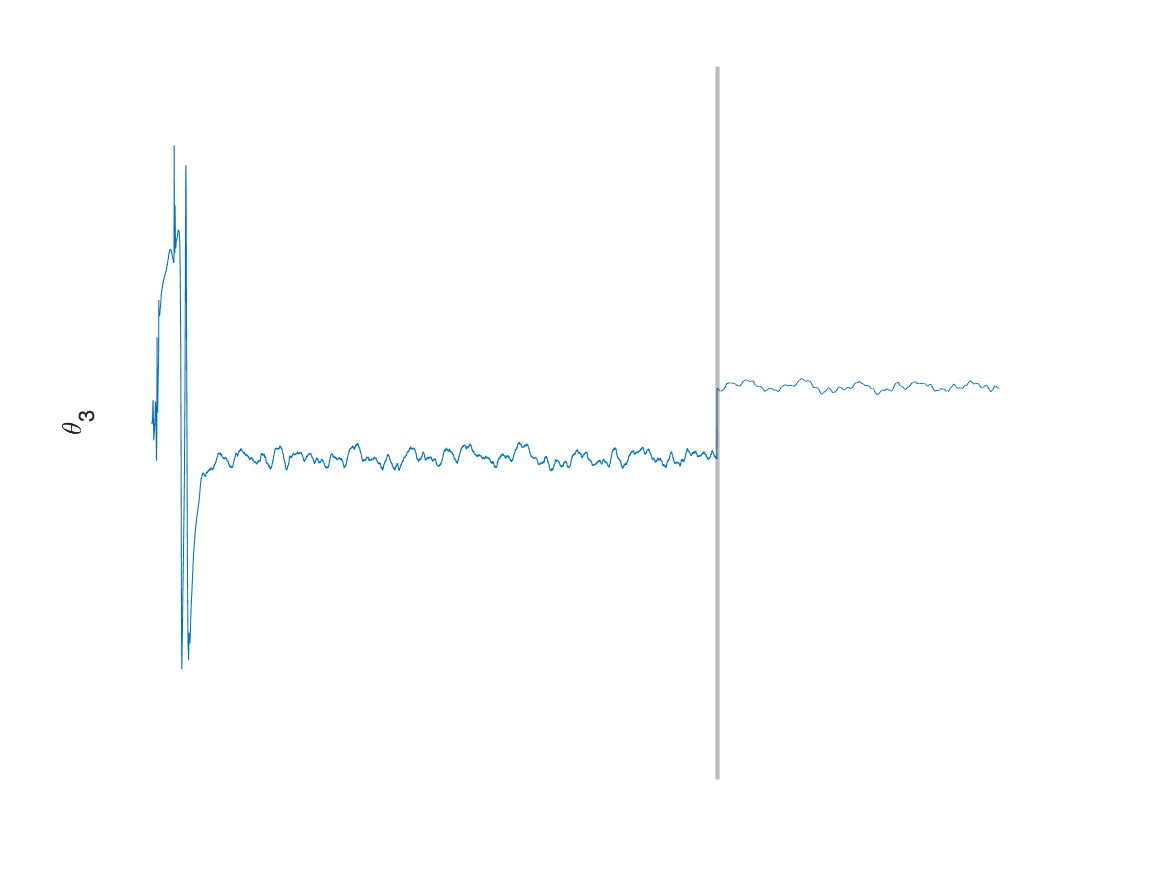
\includegraphics[height=0.1\linewidth,width=.45\linewidth]{Figures/MATLAB/ST_T3_Theta3.png}
        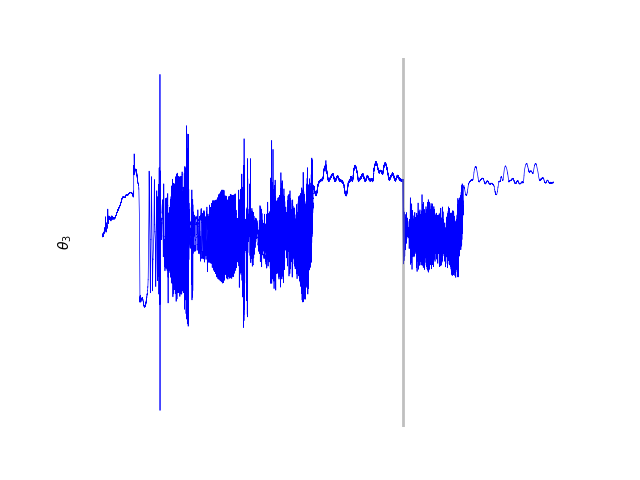
\includegraphics[height=0.1\linewidth,width=.45\linewidth]{Figures/Python/ST_T3_Theta3.png}
        
        \end{subfigure}
        

    \caption{Results for Task 3 with the SUPERTREX algorithm using the default seed (5489) for the random number generator. The target time‐series is learned accurately during the training phase, but is not maintained during the testing phase, in both implementations, in contrast to the results presented in \cite{pyle2019}.}
    \label{Fig:compTask3ST}
    
    \end{subfigure}
    
    \begin{subfigure}{\textwidth}
        \centering
        
        \textbf{\rotatebox[origin=c]{90}{SUPERTREX}}\begin{subfigure}{\textwidth}
        \centering
        
        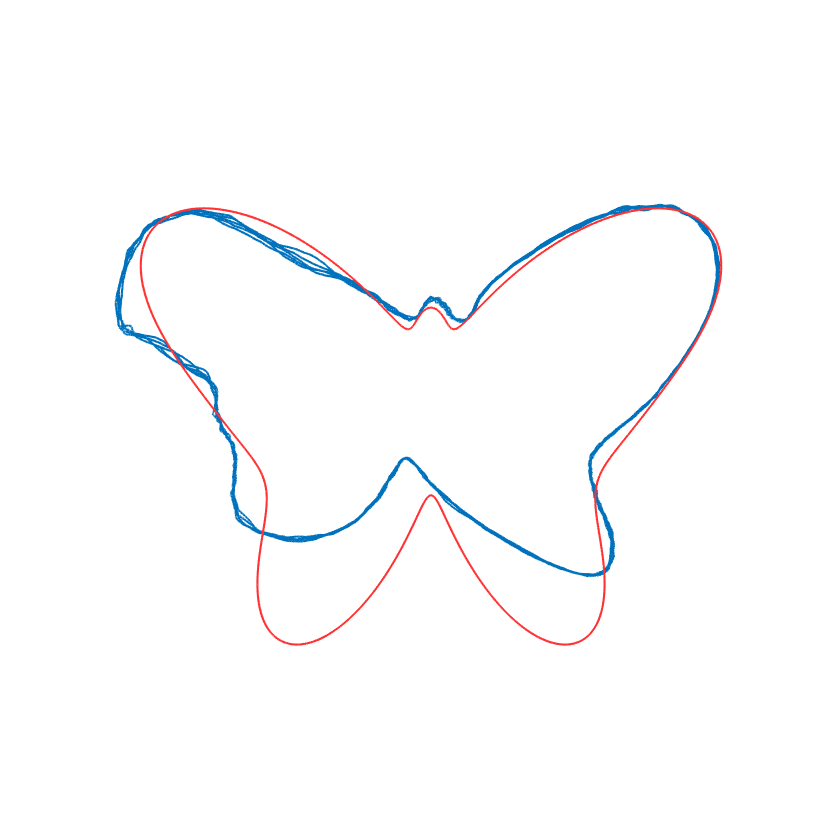
\includegraphics[trim=1.5cm 1cm 1.5cm 0cm, clip=true, height=.26\linewidth]{Figures/MATLAB/ST_T3_243454050_TimeSeries.png} 
        \hspace{2em}
        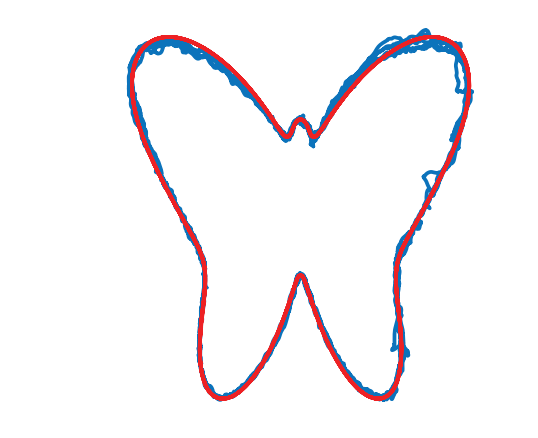
\includegraphics[height=.2\linewidth]{Figures/Orig/ST_T3_TimeSeries.png} 
        \hspace{2em}
        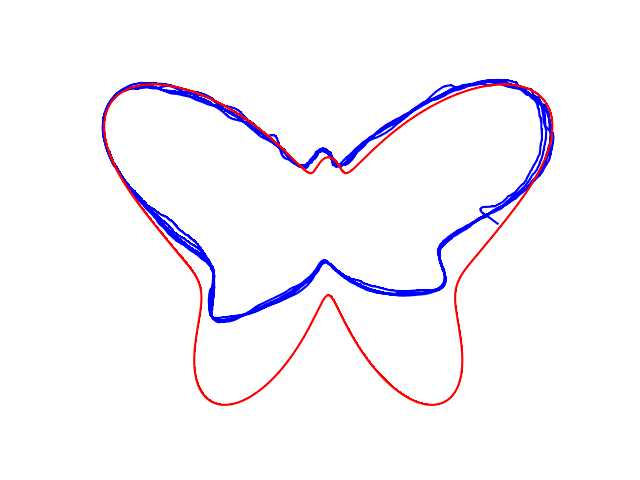
\includegraphics[trim=1.5cm 1.2cm 1.5cm 1.2cm, clip=true,  height=.2\linewidth]{Figures/Python/ST_T3_6425677_TimeSeries.png} 
        
        \end{subfigure}
        

    \caption{Results for Task 3 with the SUPERTREX algorithm using different seeds (243454050, left and 6425677, right) for the random number generator. The target time‐series is learned accurately during the training phase, and is also maintained in a stable manner, with slight divergences, during the testing phase, in both implementations, similar to the results presented in \cite{pyle2019}.}
    \label{Fig:compTask3STrseeed2}
    
    \end{subfigure}


\caption{Comparison of the performances of MATLAB (left column) and Python (right column) implementations with the results presented in the original article (center column), for two learning algorithms on task 3 \cite{pyle2019}. In each subfigure, the top panel shows the target curve (red) with the curve generated by the algorithm (blue) throughout the test phase. The bottom panel shows the actual output (blue) of the model (joint angles  ($\theta_i$), in this case) along with the target output (red), for the corresponding MATLAB (left) and Python (right) simulations. The grey vertical line demarcates the training and testing phase.}
\label{Fig:Comparison_Task3}

\end{figure}



\section{Modification}

The Python re-implementation is a close adaptation of the original MATLAB scripts provided by the authors. However, on simulating their performance on the three tasks, we observed that while, for the first two tasks, the models performed as described in \textcite{pyle2019}, the performance of the SUPERTREX algorithm on task 3 was not consistent, and was dependent on the seed used for the random number generator. On inspecting further, we notice that this was, in some cases, due to the uncontrolled exponential increase in the readout weights.\\

To verify the robustness of the implementations further, we test the performance of the RMHL and SUPERTREX algorithms on Task 2 with certain modifications to the task parameters, specifically, the number of arm segments and the length of the arm segments. It would be expected for the behaviour to be comparable with the performance on the original task performance, or undergo a gradual decline. We test Task 2 on the arm parameters, which were used in Task 3, i.e. by increasing the number of arm segments from two to three and changing the length of each arm segment. We observe that RMHL performance is comparable to the original Task 2, wherein the time series is generated during the training phase, but is not maintained beyond. However, in simulations of the SUPERTREX model, using all 11 seeds, the weights increase exponentially, rendering the simulation unable to progress in a meaningful manner . \\
    



\begin{figure}


    \centering
    
    \textbf{MATLAB}\hspace{10em}
    \textbf{Python with modification}
    
    \includegraphics[trim=1.5cm 1.4cm 1.5cm 1.2cm, clip=true, height=.25\linewidth]{Figures/MATLAB/ST_T2_Seg3_Var_TimeSeries.png}
    \hspace{8em}
    \includegraphics[ height=.25\linewidth]{Figures/Improv/ST_T2_Seg3_Var_TimeSeries.png} \\
    
    
    
    
    \textbf{\rotatebox{90}{$\theta_1$}}\begin{subfigure}{\textwidth}
        \centering
        
        \includegraphics[trim=2cm 0cm 0cm 0cm,clip=true,height=0.1\linewidth,width=.45\linewidth]{Figures/MATLAB/ST_T2_Seg3_Var_Theta1.png}
        \includegraphics[trim=2cm 0cm 0cm 0cm,clip=true,height=0.1\linewidth,width=.45\linewidth]{Figures/Improv/ST_T2_Seg3_Var_Theta1.png}            
    
    \end{subfigure}
    
    
    \textbf{\rotatebox{90}{$\theta_2$}}\begin{subfigure}{\textwidth}
        \centering
        
        \includegraphics[trim=2cm 0cm 0cm 0cm,clip=true,height=0.1\linewidth,width=.45\linewidth]{Figures/MATLAB/ST_T2_Seg3_Var_Theta2.png}
        \includegraphics[trim=2cm 0cm 0cm 0cm,clip=true,height=0.1\linewidth,width=.45\linewidth]{Figures/Improv/ST_T2_Seg3_Var_Theta2.png}           
    
    \end{subfigure}
    
    
    \textbf{\rotatebox{90}{$\theta_3$}}\begin{subfigure}{\textwidth}
        \centering
        
        \includegraphics[trim=2cm 0cm 0cm 0cm,clip=true,height=0.1\linewidth,width=.45\linewidth]{Figures/MATLAB/ST_T2_Seg3_Var_Theta3.png}
        \includegraphics[trim=2cm 0cm 0cm 0cm,clip=true,height=0.1\linewidth,width=.45\linewidth]{Figures/Improv/ST_T2_Seg3_Var_Theta3.png}           
    
    \end{subfigure}
    
    
    \textbf{\rotatebox{90}{$||W||$}}\begin{subfigure}{\textwidth}
        \centering
        
        \includegraphics[trim=1.7cm 0cm 0cm 0cm,clip=true,height=0.1\linewidth,width=.45\linewidth]{Figures/MATLAB/ST_T2_Seg3_Var_W_norm.png}
        \includegraphics[trim=1.2cm 0cm 0cm 0cm,clip=true,height=0.1\linewidth,width=.45\linewidth]{Figures/Improv/ST_T2_Seg3_Var_W_norm.png}              
    
    \end{subfigure}
        
            



\caption{Robustness of the SUPERTREX model on a Task 2 variant. The performance of the MATLAB (left column) and modified Python implementations (right column) is tested for the SUPERTREX learning algorithm on a variant of Task 2 with increased number of arm segments (lengths: 1.8, 1.2, 0.6). The top panel shows the target curve (red) with the curve generated by the algorithm (blue) throughout the test phase. The bottom panel shows the actual output (blue) of the model (joint angles  ($\theta_i$), in this case) along with the target output (red), for the corresponding MATLAB (left) and Python (right) simulations. The grey vertical line demarcates the training and testing phase. In the original MATLAB scripts, the readout weights increase uncontrollably rendering the model unable to learn. The Python adaptation, using  a compensation factor to harness the weight update, is able to learn and converge to produce the target timeseries.}
\label{Fig:Comparison_Task2_Seg3}

\end{figure}


In order to make the model more scalable in terms of task parameters, and also more robust (as seen in Task 3, with respect to reproducibility with different random seeds), we introduce two minor alterations.

\begin{itemize}
    \item One, we introduce a compensation factor to the update of the readout weights in the exploratory pathway, inversely proportional to the number of segments. Specifically, when the number of segments is greater than two, we multiply the weight update by $0.1/n\_segs$ for Task 2 and by $0.5/n\_segs$ for Task 3.
    \item Two, the SUPERTREX model transfers the information from the exploratory pathway to the mastery pathway, only if the error is consistently below a certain threshold. In the MATLAB scripts, this threshold is set at 1.5e-3 for Task 1 and Task 2, while at 1.5e-2 for Task 3. We change the transfer threshold for Task 2 from 1.5e-3 to 1.5e-2. 
\end{itemize}

These slight modifications address the minor shortcomings we encountered earlier with the performance of SUPERTREX in Task 2 and 3, by including a compensation factor for the change in number of arm segments. This prevents the weights from increasing exponentially, and lets the simulation proceed in a meaningful manner. We also increase the error threshold governing the transfer of information to the mastery pathway. The increase from 1.5e-3 to 1.5e-2 makes the model more tolerant of fluctuations, while continuing to explore and learn a good solution. Although this does not lead to a critical change for the above tasks, this alteration unlocks the potential for the model to be more scalable. We find that with these alterations, on merely increasing the number of timesteps per training cycle and with no further fine tuning of hyperparameters, the model is able to learn with reasonable accuracy over a wider range of task parameters, for e.g., on adding surplus segments with length 0.1 each, the model is able to perform well with up to 50 arm segments  (Figure~\ref{Fig:Scalability_Task2}).







\begin{figure}

        \textbf{\rotatebox[origin=c]{90}{\hspace{-7.5em} MSE \hspace{2.5em} y(t) \hspace{1.5em} x(t)}}
        \begin{subfigure}{\textwidth}
            \centering
    
            \textbf{5 segments}\hspace{12em}\textbf{6 segments}
            
            \includegraphics[height=0.15\linewidth]{Figures/Improv/ST_T2_Seg5_Var_TimeSeries.png}
            \hspace{9em}
            \includegraphics[height=0.15\linewidth]{Figures/Improv/ST_T2_Seg6_Var_TimeSeries.png}\\
            
            \includegraphics[trim=2cm 0cm 0cm 0cm, clip=true,height=0.1\linewidth,width=.45\linewidth]{Figures/Improv/ST_T2_Seg5_Var_CoordinateX.png}         
            \includegraphics[trim=2cm 0cm 0cm 0cm, clip=true,height=0.1\linewidth,width=.45\linewidth]{Figures/Improv/ST_T2_Seg6_Var_CoordinateX.png}         

            \includegraphics[trim=2cm 0cm 0cm 0cm, clip=true,height=0.1\linewidth,width=.45\linewidth]{Figures/Improv/ST_T2_Seg5_Var_CoordinateY.png}         
            \includegraphics[trim=2cm 0cm 0cm 0cm, clip=true,height=0.1\linewidth,width=.45\linewidth]{Figures/Improv/ST_T2_Seg6_Var_CoordinateY.png}         

            \includegraphics[trim=1cm 0cm 0cm 0cm, clip=true,height=0.1\linewidth,width=.45\linewidth]{Figures/Improv/ST_T2_Seg5_Var_MSE.png}
            \includegraphics[trim=1cm 0cm 0cm 0cm, clip=true,height=0.1\linewidth,width=.45\linewidth]{Figures/Improv/ST_T2_Seg6_Var_MSE.png}

        \end{subfigure}
        
        \textbf{\rotatebox[origin=c]{90}{\hspace{-7.5em} MSE \hspace{2.5em} y(t) \hspace{1.5em} x(t)}}
        \begin{subfigure}{\textwidth}
            \centering
    
            \textbf{7 segments}\hspace{12em}\textbf{8 segments}
            
            \includegraphics[height=0.15\linewidth]{Figures/Improv/ST_T2_Seg7_Var_TimeSeries.png}
            \hspace{9em}
            \includegraphics[height=0.15\linewidth]{Figures/Improv/ST_T2_Seg8_Var_TimeSeries.png}\\
            
            \includegraphics[trim=2cm 0cm 0cm 0cm, clip=true,height=0.1\linewidth,width=.45\linewidth]{Figures/Improv/ST_T2_Seg7_Var_CoordinateX.png}
            \includegraphics[trim=2cm 0cm 0cm 0cm, clip=true,height=0.1\linewidth,width=.45\linewidth]{Figures/Improv/ST_T2_Seg8_Var_CoordinateX.png}         
       
                    
            \includegraphics[trim=2cm 0cm 0cm 0cm, clip=true,height=0.1\linewidth,width=.45\linewidth]{Figures/Improv/ST_T2_Seg7_Var_CoordinateY.png}         
            \includegraphics[trim=2cm 0cm 0cm 0cm, clip=true,height=0.1\linewidth,width=.45\linewidth]{Figures/Improv/ST_T2_Seg8_Var_CoordinateX.png}         
           
            \includegraphics[trim=1cm 0cm 0cm 0cm, clip=true,height=0.1\linewidth,width=.45\linewidth]{Figures/Improv/ST_T2_Seg7_Var_MSE.png}
            \includegraphics[trim=1cm 0cm 0cm 0cm, clip=true,height=0.1\linewidth,width=.45\linewidth]{Figures/Improv/ST_T2_Seg8_Var_MSE.png}
            
        \end{subfigure}
        
        \textbf{\rotatebox[origin=c]{90}{\hspace{-7.5em} MSE \hspace{2.5em} y(t) \hspace{1.5em} x(t)}}
        \begin{subfigure}{\textwidth}
            \centering
    
            \textbf{9 segments}\hspace{12em}\textbf{10 segments}
            
            \includegraphics[height=0.15\linewidth]{Figures/Improv/ST_T2_Seg9_Var_TimeSeries.png}
            \hspace{9em}
            \includegraphics[height=0.15\linewidth]{Figures/Improv/ST_T2_Seg10_Var_TimeSeries.png}\\

            \includegraphics[trim=2cm 0cm 0cm 0cm, clip=true,height=0.1\linewidth,width=.45\linewidth]{Figures/Improv/ST_T2_Seg9_Var_CoordinateX.png}         
            \includegraphics[trim=2cm 0cm 0cm 0cm, clip=true,height=0.1\linewidth,width=.45\linewidth]{Figures/Improv/ST_T2_Seg10_Var_CoordinateX.png}         
            
            \includegraphics[trim=2cm 0cm 0cm 0cm, clip=true,height=0.1\linewidth,width=.45\linewidth]{Figures/Improv/ST_T2_Seg9_Var_CoordinateX.png}         
            \includegraphics[trim=2cm 0cm 0cm 0cm, clip=true,height=0.1\linewidth,width=.45\linewidth]{Figures/Improv/ST_T2_Seg10_Var_CoordinateX.png}   
            
            
            \includegraphics[trim=1cm 0cm 0cm 0cm, clip=true,height=0.1\linewidth,width=.45\linewidth]{Figures/Improv/ST_T2_Seg9_Var_MSE.png}
            \includegraphics[trim=1cm 0cm 0cm 0cm, clip=true,height=0.1\linewidth,width=.45\linewidth]{Figures/Improv/ST_T2_Seg10_Var_MSE.png}
            
        \end{subfigure}
    \caption{Scalability of the performance of the modified Python implementation using the SUPERTREX algorithm on Task 2. The lengths of the arm segments are 1.8, 1.2 and 0.6 for the first three segments. (akin to task 3) and 0.1 for each additional segment. Here, the simulations for task 2 with 5 to 50 segments are shown, all using the default seed 5489 for the random number generator. In each subfigure, the top panel shows the produced curve, the middle panels show the evolution of the x and y coordinates of the end-effector of the arm (blue) throughout the training and test phase, along with the target (red). The grey vertical line demarcates the training and testing phase. The bottom panel shows the progression of the mean squared error through the simulation. Until ten segments, we use 10000 timesteps per cycle, 15000 for twenty segments, 20000 for thirty to forty segments and 30000 for fifty segments. Without any further parameter tuning, the model is able to learn to generate the timeseries with an arm composed of upto 50 segments, albeit with lower precision. (Continued on next page.)}
    \label{Fig:Scalability_Task2}

\end{figure}
    
    
\begin{figure}
\ContinuedFloat
        \textbf{\rotatebox[origin=c]{90}{\hspace{-7.5em} MSE \hspace{2.5em} y(t) \hspace{1.5em} x(t)}}
        \begin{subfigure}{\textwidth}
            \centering
    
            \textbf{20 segments}\hspace{12em}\textbf{30 segments}
            
            \includegraphics[height=0.15\linewidth]{Figures/Improv/ST_T2_Seg20_Var_TimeSeries.png}
            \hspace{9em}
            \includegraphics[height=0.15\linewidth]{Figures/Improv/ST_T2_Seg30_Var_TimeSeries.png}\\

            \includegraphics[trim=2cm 0cm 0cm 0cm, clip=true,height=0.1\linewidth,width=.45\linewidth]{Figures/Improv/ST_T2_Seg20_Var_CoordinateX.png}        
            \includegraphics[trim=2cm 0cm 0cm 0cm, clip=true,height=0.1\linewidth,width=.45\linewidth]{Figures/Improv/ST_T2_Seg30_Var_CoordinateX.png}         

            \includegraphics[trim=2cm 0cm 0cm 0cm, clip=true,height=0.1\linewidth,width=.45\linewidth]{Figures/Improv/ST_T2_Seg20_Var_CoordinateX.png}        
            \includegraphics[trim=2cm 0cm 0cm 0cm, clip=true,height=0.1\linewidth,width=.45\linewidth]{Figures/Improv/ST_T2_Seg30_Var_CoordinateX.png}         

            \includegraphics[trim=1cm 0cm 0cm 0cm, clip=true,height=0.1\linewidth,width=.45\linewidth]{Figures/Improv/ST_T2_Seg20_Var_MSE.png}
            \includegraphics[trim=1cm 0cm 0cm 0cm, clip=true,height=0.1\linewidth,width=.45\linewidth]{Figures/Improv/ST_T2_Seg30_Var_MSE.png}

        \end{subfigure}
        
        \textbf{\rotatebox[origin=c]{90}{\hspace{-7.5em} MSE \hspace{2.5em} y(t) \hspace{1.5em} x(t)}}
        \begin{subfigure}{\textwidth}
            \centering
    
            \textbf{40 segments}\hspace{12em}\textbf{50 segments}
            
            \includegraphics[height=0.15\linewidth]{Figures/Improv/ST_T2_Seg40_Var_TimeSeries.png}
            \hspace{10em}
            \includegraphics[height=0.15\linewidth]{Figures/Improv/ST_T2_Seg50_Var_TimeSeries.png}\\


            \includegraphics[trim=2cm 0cm 0cm 0cm, clip=true,height=0.1\linewidth,width=.45\linewidth]{Figures/Improv/ST_T2_Seg40_Var_CoordinateX.png}
            \includegraphics[trim=2cm 0cm 0cm 0cm, clip=true,height=0.1\linewidth,width=.45\linewidth]{Figures/Improv/ST_T2_Seg50_Var_CoordinateX.png}         

            \includegraphics[trim=2cm 0cm 0cm 0cm, clip=true,height=0.1\linewidth,width=.45\linewidth]{Figures/Improv/ST_T2_Seg40_Var_CoordinateX.png}    
            \includegraphics[trim=2cm 0cm 0cm 0cm, clip=true,height=0.1\linewidth,width=.45\linewidth]{Figures/Improv/ST_T2_Seg50_Var_CoordinateX.png}         
            
            \includegraphics[trim=1cm 0cm 0cm 0cm, clip=true,height=0.1\linewidth,width=.45\linewidth]{Figures/Improv/ST_T2_Seg40_Var_MSE.png}
            \includegraphics[trim=1cm 0cm 0cm 0cm, clip=true,height=0.1\linewidth,width=.45\linewidth]{Figures/Improv/ST_T2_Seg50_Var_MSE.png}
            
        \end{subfigure}
    


    \caption{(Continued from previous page.) Scalability of the performance of the modified Python implementation using the SUPERTREX algorithm on Task 2. The lengths of the arm segments are 1.8, 1.2 and 0.6 for the first three segments. (akin to task 3) and 0.1 for each additional segment. Here, the simulations for task 2 with 5 to 50 segments are shown, all using the default seed 5489 for the random number generator. In each subfigure, the top panel shows the produced curve, the middle panels show the evolution of the x and y coordinates of the end-effector of the arm (blue) throughout the training and test phase, along with the target (red). The grey vertical line demarcates the training and testing phase. The bottom panel shows the progression of the mean squared error through the simulation. Until ten segments, we use 10000 timesteps per cycle, 15000 for twenty segments, 20000 for thirty to forty segments and 30000 for fifty segments. Without any further parameter tuning, the model is able to learn to generate the timeseries with an arm composed of upto 50 segments, albeit with lower precision.}
    \label{Fig:Scalability_Task2_cont}

\end{figure}



\section{Discussion}

In this article, we discussed the SUPERTREX model presented by
\textcite{pyle2019}. We compared the results presented in the paper
using the MATLAB scripts provided by the author with out modular and
user-friendly Python replication. Furthermore, we were able to improve
the robustness and scalability of the model with two minor alterations,
%
The Python re-implementation strives to be a close adaptation of the
original scripts of the authors and differs mainly in the method of
initialisation of the reservoir connectivity matrix. This is due to
the usage of the function {\tt sprandn} in the MATLAB scripts, whose
internal implementation is freely available. Most of the details for
the implementation of the models are also described in the paper. Only
two necessary details were missing, the inclusion of a crucial
learning rate of 0.0005 and a compensatory factor of 0.5 within the
update of the readout weights of the exploratory pathway in the RMHL
and SUPERTREX models for Tasks 2 and 3.
%
The three algorithms (FORCE, RMHL and SUPERTREX) have been tested on
three tasks, presented in \textcite{pyle2019}. For Task 1 and 2, we
can now confirm that the three algorithms function as presented in the
paper. For Task 3, the SUPERTREX model's behaviour is also
reproducible, although the performance is dependent on the seed used
for the random number generator. Furthermore, we observed that the
model is quite sensitive to changes in task parameters, such as the
number of arms. In several cases, this was due to the uninhibited
increase in the readout weights. We propose the inclusion of a
compensation factor for the number of arm segments, which limits the
growth of the readout weights, and allows the simulation to proceed in
a meaningful manner. This considerably improves the robustness and the
scalability of the original model.\\

We can conclude that the theory is promising and the model functions
as presented in the paper for Task 1 and 2, and with a minor adjustment
for task 3.


% ----------------------------------------------
